\documentclass[]{book}
\usepackage{lmodern}
\usepackage{amssymb,amsmath}
\usepackage{ifxetex,ifluatex}
\usepackage{fixltx2e} % provides \textsubscript
\ifnum 0\ifxetex 1\fi\ifluatex 1\fi=0 % if pdftex
  \usepackage[T1]{fontenc}
  \usepackage[utf8]{inputenc}
\else % if luatex or xelatex
  \ifxetex
    \usepackage{mathspec}
  \else
    \usepackage{fontspec}
  \fi
  \defaultfontfeatures{Ligatures=TeX,Scale=MatchLowercase}
\fi
% use upquote if available, for straight quotes in verbatim environments
\IfFileExists{upquote.sty}{\usepackage{upquote}}{}
% use microtype if available
\IfFileExists{microtype.sty}{%
\usepackage{microtype}
\UseMicrotypeSet[protrusion]{basicmath} % disable protrusion for tt fonts
}{}
\usepackage[unicode=true]{hyperref}
\hypersetup{
            pdfborder={0 0 0},
            breaklinks=true}
\urlstyle{same}  % don't use monospace font for urls
\usepackage{color}
\usepackage{fancyvrb}
\newcommand{\VerbBar}{|}
\newcommand{\VERB}{\Verb[commandchars=\\\{\}]}
\DefineVerbatimEnvironment{Highlighting}{Verbatim}{commandchars=\\\{\}}
% Add ',fontsize=\small' for more characters per line
\usepackage{framed}
\definecolor{shadecolor}{RGB}{248,248,248}
\newenvironment{Shaded}{\begin{snugshade}}{\end{snugshade}}
\newcommand{\KeywordTok}[1]{\textcolor[rgb]{0.13,0.29,0.53}{\textbf{{#1}}}}
\newcommand{\DataTypeTok}[1]{\textcolor[rgb]{0.13,0.29,0.53}{{#1}}}
\newcommand{\DecValTok}[1]{\textcolor[rgb]{0.00,0.00,0.81}{{#1}}}
\newcommand{\BaseNTok}[1]{\textcolor[rgb]{0.00,0.00,0.81}{{#1}}}
\newcommand{\FloatTok}[1]{\textcolor[rgb]{0.00,0.00,0.81}{{#1}}}
\newcommand{\ConstantTok}[1]{\textcolor[rgb]{0.00,0.00,0.00}{{#1}}}
\newcommand{\CharTok}[1]{\textcolor[rgb]{0.31,0.60,0.02}{{#1}}}
\newcommand{\SpecialCharTok}[1]{\textcolor[rgb]{0.00,0.00,0.00}{{#1}}}
\newcommand{\StringTok}[1]{\textcolor[rgb]{0.31,0.60,0.02}{{#1}}}
\newcommand{\VerbatimStringTok}[1]{\textcolor[rgb]{0.31,0.60,0.02}{{#1}}}
\newcommand{\SpecialStringTok}[1]{\textcolor[rgb]{0.31,0.60,0.02}{{#1}}}
\newcommand{\ImportTok}[1]{{#1}}
\newcommand{\CommentTok}[1]{\textcolor[rgb]{0.56,0.35,0.01}{\textit{{#1}}}}
\newcommand{\DocumentationTok}[1]{\textcolor[rgb]{0.56,0.35,0.01}{\textbf{\textit{{#1}}}}}
\newcommand{\AnnotationTok}[1]{\textcolor[rgb]{0.56,0.35,0.01}{\textbf{\textit{{#1}}}}}
\newcommand{\CommentVarTok}[1]{\textcolor[rgb]{0.56,0.35,0.01}{\textbf{\textit{{#1}}}}}
\newcommand{\OtherTok}[1]{\textcolor[rgb]{0.56,0.35,0.01}{{#1}}}
\newcommand{\FunctionTok}[1]{\textcolor[rgb]{0.00,0.00,0.00}{{#1}}}
\newcommand{\VariableTok}[1]{\textcolor[rgb]{0.00,0.00,0.00}{{#1}}}
\newcommand{\ControlFlowTok}[1]{\textcolor[rgb]{0.13,0.29,0.53}{\textbf{{#1}}}}
\newcommand{\OperatorTok}[1]{\textcolor[rgb]{0.81,0.36,0.00}{\textbf{{#1}}}}
\newcommand{\BuiltInTok}[1]{{#1}}
\newcommand{\ExtensionTok}[1]{{#1}}
\newcommand{\PreprocessorTok}[1]{\textcolor[rgb]{0.56,0.35,0.01}{\textit{{#1}}}}
\newcommand{\AttributeTok}[1]{\textcolor[rgb]{0.77,0.63,0.00}{{#1}}}
\newcommand{\RegionMarkerTok}[1]{{#1}}
\newcommand{\InformationTok}[1]{\textcolor[rgb]{0.56,0.35,0.01}{\textbf{\textit{{#1}}}}}
\newcommand{\WarningTok}[1]{\textcolor[rgb]{0.56,0.35,0.01}{\textbf{\textit{{#1}}}}}
\newcommand{\AlertTok}[1]{\textcolor[rgb]{0.94,0.16,0.16}{{#1}}}
\newcommand{\ErrorTok}[1]{\textcolor[rgb]{0.64,0.00,0.00}{\textbf{{#1}}}}
\newcommand{\NormalTok}[1]{{#1}}
\usepackage{longtable,booktabs}
\usepackage{graphicx,grffile}
\makeatletter
\def\maxwidth{\ifdim\Gin@nat@width>\linewidth\linewidth\else\Gin@nat@width\fi}
\def\maxheight{\ifdim\Gin@nat@height>\textheight\textheight\else\Gin@nat@height\fi}
\makeatother
% Scale images if necessary, so that they will not overflow the page
% margins by default, and it is still possible to overwrite the defaults
% using explicit options in \includegraphics[width, height, ...]{}
\setkeys{Gin}{width=\maxwidth,height=\maxheight,keepaspectratio}
\IfFileExists{parskip.sty}{%
\usepackage{parskip}
}{% else
\setlength{\parindent}{0pt}
\setlength{\parskip}{6pt plus 2pt minus 1pt}
}
\setlength{\emergencystretch}{3em}  % prevent overfull lines
\providecommand{\tightlist}{%
  \setlength{\itemsep}{0pt}\setlength{\parskip}{0pt}}
\setcounter{secnumdepth}{5}
% Redefines (sub)paragraphs to behave more like sections
\ifx\paragraph\undefined\else
\let\oldparagraph\paragraph
\renewcommand{\paragraph}[1]{\oldparagraph{#1}\mbox{}}
\fi
\ifx\subparagraph\undefined\else
\let\oldsubparagraph\subparagraph
\renewcommand{\subparagraph}[1]{\oldsubparagraph{#1}\mbox{}}
\fi

\author{}
\date{\vspace{-2.5em}}

\begin{document}

{
\setcounter{tocdepth}{1}
\tableofcontents
}
\chapter{Thurs Sept 10: Syllabus}\label{thurs-sept-10-syllabus}

\section{Instructor Information}\label{instructor-information}

Instructor: Dr.~Amy Hurford\\
Office: Teaching remotely\\
Email: \href{mailto:ahurford@mun.ca}{\nolinkurl{ahurford@mun.ca}}\\
I will try to reply to emails within 24 hours (excluding evenings,
weekends and holidays). I am always available during the lecture times.
Please email to request a meeting for a different time. Please check my
\href{https://amyhurford.weebly.com/}{schedule} and suggest a time I am
free that works for you.

\section{Course Information}\label{course-information}

TR 12.00-12.50pm\\
F 1-1.50pm\\
WebEx links for lecture times are on the course Brightspace under
Announcements.

Course description:\\
Population and Evolutionary Ecology is an introduction to the theory and
principles of evolutionary ecology and population dynamics.
Pre-requisites: BIOL 2600; at least one of BIOL 2010, 2122 or
2210.\\[2\baselineskip]Course format:\\
The course has been re-designed for online delivery. Specifically, no
exams that require invigilation are part of the grading scheme because
these are challenging to deliver remotely. Pre-recorded lectures limit
my ability to interact with students. Therefore, I have elected to
dedicate all lecture time to interacting with students. For each class
there is a list of questions you are required to answer and hand-in.
Prior to some classes there may be a \emph{Required Reading}, that if
completed will allow you to answer the day's assignment questions. Prior
to the day of class you should complete the \emph{Required Reading}. In
addition, I can most effectively help you if you have read over the
questions ahead of time.

Course expectations:\\
Any students that are disruptive, violating university policies, or
acting in a potentially unsafe way will be warned and asked to
leave.\\[2\baselineskip]Learning goals:\\
I consider your completed assignments to be a portfolio of your
knowledge in population and evolutionary ecology. You will also get some
exposure to coding in \texttt{R}. It takes time to become proficient in
a programming language, but the time you will spend coding in this class
will help you towards becoming more proficient. The course content
emphasizes a deeper understanding of fewer concepts. You have the
opportunity to further explore a topic of interest to you for the final
project.

Required Text and Resources:\\
The course materials are online at
\url{https://ahurford.github.io/BIOL-3295-Fall-2020/}. In addition you
will need a computer to install \texttt{R} and \texttt{RStudio}. This
will be covered on Thursday Sept 17 (see Chapter \ref{Rinstall}). Class
announcements and WebEx links will be provided on the course BrightSpace
and your assignments are to be submitted to BrightSpace.

\section{Method of Evaluation}\label{method-of-evaluation}

\begin{itemize}
\tightlist
\item
  27 assignments (equal weighting) - 50\%
\item
  Midterm (due Fri Nov 6 at 5pm) - 15\%
\item
  Final Project (due Monday Dec 14 at 9am) - 35\%
\end{itemize}

You should aim to complete each assignment before the next class, but
assignments will be accepted, without penalty, up to a week later.

Late assignments, labs, and missed midterms, and final exams will be
accommodated as described by University Regulation 6.7.3 and 6.7.5 (see
\url{https://www.mun.ca/regoff/calendar/sectionNo=REGS-0474} for
Regulations).

\section{Additional Policies}\label{additional-policies}

\subsection{Accommodation of students with
disabilities}\label{accommodation-of-students-with-disabilities}

Memorial University of Newfoundland is committed to supporting inclusive
education based on the principles of equity, accessibility and
collaboration. Accommodations are provided within the scope of the
University Policies for the Accommodations for Students with
Disabilities see \url{www.mun.ca/policy/site/policy.php?id=239}.
Students who may need an academic accommodation are asked to initiate
the request with the Glenn Roy Blundon Centre at the earliest
opportunity (see \url{www.mun.ca/blundon} for more information).

\subsection{Academic misconduct}\label{academic-misconduct}

Students are expected to adhere to those principles, which constitute
proper academic conduct. A student has the responsibility to know which
actions, as described under Academic Offences in the University
Regulations, could be construed as dishonest or improper. Students found
guilty of an academic offence may be subject to a number of penalties
commensurate with the offence including reprimand, reduction of grade,
probation, suspension or expulsion from the University. For more
information regarding this policy, students should refer to University
Regulation 6.12.

\subsection{Equity and Diversity}\label{equity-and-diversity}

A safe learning environment will be provided for all students regardless
of race, colour, nationality, ethnic origin, social origin, religious
creed, religion, age, disability, disfigurement, sex (including
pregnancy), sexual orientation, gender identity, gender expression,
marital status, family status, source of income or political opinion.

You should not photograph or record myself, teaching assistants, or
other students in the class without first obtaining permission.
Accommodation will be made for students with special needs.

The sound should be turned off on phones and computers during class.

\section{Additional Supports}\label{additional-supports}

Resources for additional support can be found at:

\begin{itemize}
\item
  \url{www.mun.ca/currentstudents/student/}
\item
  \url{https://munsu.ca/resource-centres/}
\end{itemize}

\section{Tentative course schedule}\label{tentative-course-schedule}

The course schedule is found in the toolbar of the class materials, see
\url{https://ahurford.github.io/BIOL-3295-Fall-2020/}.

The last day to drop the course without academic prejudice is Wednesday
Nov. 4.

\section{Handing in your work}\label{handing-in-your-work}

\subsection{Making figures to hand-in}\label{figures}

The graphs you hand in need to have descriptive axeses and a figure
caption. You may put these elements together using a word processing
software such as \emph{Microsoft Word}. Elements of a good figure
caption:

\begin{itemize}
\item
  Has a label, i.e., ``Figure 1'',
\item
  The first sentences provides a summary of what the figure shows, i.e.,
  ``The price of oranges has increased steadily since 1964'',
\item
  Provide all necessary information to understand everything in the
  figure, i.e., if the figure has no legend, but multiple line
  types/symbols, be sure to indicate what is represented by the
  different symbols. If the axes labels are overly brief due to space
  constraints in the graph, provide a more thorough description in the
  figure caption. If any assumptions have been made in making the
  figure, disclose these, i.e., a point that was excluded from the
  analysis due to being considered an outlier.
\end{itemize}

\subsection{Writing R scripts to hand-in}\label{RScript}

To write your own R scripts follow the guidelines described in Chapter 7
\href{https://ahurford.github.io/quant-guide-all-courses/style.html}{Best
Practices} of \emph{Quantitative training in Biology}. If you are asked
to hand in your R script this means you need to submit an \texttt{.R}
file on Brightspace.

\chapter{Friday Sept 11: What is a
population?}\label{friday-sept-11-what-is-a-population}

For the questions below, submit your answers to Brightspace ideally
before the next class. The deadline to submit your answers is Friday
Sept 18.

The \emph{Resources} below are sufficient to answer all the questions,
however, you are encouraged to find your own textbooks or peer-reviewed
articles to answer the questions if you feel comfortable. You can search
for textbooks using and the \href{https://www.library.mun.ca/}{library
catalogue} and peer-reviewed articles using
\href{https://apps-webofknowledge-com.qe2a-proxy.mun.ca/WOS_GeneralSearch_input.do?product=WOS\&search_mode=GeneralSearch\&SID=5COlVVH7qj2puc72yvk\&preferencesSaved=}{Web
of Science}.

\section{Questions}\label{questions}

\begin{enumerate}
\def\labelenumi{\arabic{enumi}.}
\item
  Give a definition of a population from a textbook or peer-reviewed
  publication. Provide the citation. {[}2 marks{]}
\item
  Find a peer-reviewed paper where a population is studied. Write 1
  paragraph discussing how a population is defined for the study and how
  this compares to your definition of a population given in Question 1.
  {[}5 marks{]}
\end{enumerate}

\section{Resources}\label{resources}

Vandermeer, J.H., Goldberg, D.E., 2013. Population Ecology: First
Principles (Second Edition). Princeton University Press, Princeton,
United States.
\href{https://ebookcentral-proquest-com.qe2a-proxy.mun.ca/lib/mun/detail.action?docID=1205619}{Link}

The Princeton Guide to Ecology, edited by Simon A. Levin, et al.,
Princeton University Press, 2009. ProQuest Ebook Central,
\href{https://ebookcentral-proquest-com.qe2a-proxy.mun.ca/lib/mun/detail.action?docID=557123}{Link}

Sacchi, R., Gentilli, A., Razzetti, E., Barbieri, F., 2002. Effects of
building features on density and flock distribution of feral pigeons
Columba livia var. domestica in an urban environment. Can. J. Zool. 80,
48-54. \href{https://doi.org/10.1139/z01-202}{Link}

\chapter{Tues Sept 15: Exponential growth - discrete
time}\label{tues-sept-15-exponential-growth---discrete-time}

Please submit your answers before the next class. You have until Tues
Sept 22 to submit your answers.

\section{Required reading}\label{required-reading}

Vandermeer, J.H., Goldberg, D.E., 2013. Population Ecology: First
Principles (Second Edition). Princeton University Press, Princeton,
United States. p1-3.
\href{https://ebookcentral-proquest-com.qe2a-proxy.mun.ca/lib/mun/detail.action?docID=1205619}{Link}

\section{Questions}\label{questions}

\begin{enumerate}
\def\labelenumi{\arabic{enumi}.}
\item
  Suppose \(\lambda = 5\) in equation (3) (see the required reading).
  Explain in 1-2 sentences the meaning of \(\lambda = 5\). {[}1 mark{]}
\item
  Suppose the number of lilypads during week 7 is 78,125. Let
  \(\lambda = 5\), and assume that the units of \(t\) are weeks. Use
  equation (3) to calculate the number of lilypads in week 8. Show your
  calculations. {[}2 marks{]}
\item
  Use your answer to question 2. to calculate the number of lilypads in
  week 9. Show your calculations. {[}2 marks{]}
\item
  Equation (4) for the required reading assumes that \(N_0=1\), however,
  this formula can be generalized such that
\end{enumerate}

\[
N_t = N_0\lambda^t
\]

where \(N_t\) is the population size at time, \(t\). Define time such
that \(t=0\) is week 7 and \(t\) is then the number of weeks since week
7. Use the equation above to answer question 3 and confirm that the
answer is the same (i.e., find the population size for week 9, when
\(\lambda=5\) and the population size for week 7 is 78,125). Show your
calculations. {[}2 marks{]}

\begin{enumerate}
\def\labelenumi{\arabic{enumi}.}
\setcounter{enumi}{4}
\item
  Use the formula from question 4 to find the population size for week
  15, where \(N_0=1\) and \(\lambda=5\). {Define time as the number of
  weeks since week 0}. Show your calculations {[}2 marks{]}
\item
  It is important to note that all mathematical formulas should have the
  same units on both sides of the equals sign, and for each term that is
  added or subtracted. The units of the population size, \(N_t\), at
  time, \(t\), are number. The geometric growth rate, \(\lambda\) is
  unitless. Choose an equation from the required reading and give the
  units for each of the terms to show that both sides of the equals have
  the same units. For example, for the equation that appears in question
  4, we have:
\end{enumerate}

\begin{eqnarray*}
N_t & = & N_0 \lambda^t \\
\left(\mbox{number}\right)& =&(\mbox{number}) (\mbox{unitless})^{weeks}\\
\left(\mbox{number}\right)& =& \left(\mbox{number}\right)\\
\end{eqnarray*}

Note that:

\begin{eqnarray*}
(\mbox{unitless}) \times (\mbox{quantity with units}) & = & (\mbox{quantity with units}) \\ (\mbox{unitless})^{(\mbox{quantity})}& =& (\mbox{unitless})
\end{eqnarray*}

{[}2 marks{]}

\begin{enumerate}
\def\labelenumi{\arabic{enumi}.}
\setcounter{enumi}{6}
\item
  Although not stated in the reading, \(\lambda = 1 + b - d\) where
  \(b\) is the per capita birth rate over one time step (i.e.~one week
  for this example), and \(d\) is the fraction of the lilypad population
  that dies over one time step. The number 1 is considered unitless,
  what must the units of \(b\) and \(d\) be? {[}1 mark{]}
\item
  In the reading, \(\lambda = 2\). Given that \(\lambda = 1 + b - d\),
  what are some possible values of \(b\) and \(d\). {Note that \(d\) is
  a fraction and must be \(1 \geq d \geq 0\) and \(b>0\).} {[}1 mark{]}
\item
  {[}True or False{]} For discrete time exponential growth (as per the
  reading), the change in population size from one week to the next
  depends not so much on the per capita birth rate, but on the
  difference between the per capita birth rate and the per capita death
  rate. {[}1 mark{]}
\end{enumerate}

\chapter{Thurs Sept 17: Getting started with R}\label{Rinstall}

You need to have the \texttt{R} and \texttt{RStudio} softwares installed
before you can proceed with the next class. Your answer to the question
is due Thursday Sept 24.

\section{Required reading}\label{required-reading}

You are required to read and complete all the exercises in Chapters 1
\href{https://ahurford.github.io/quant-guide-all-courses/}{\emph{Introduction}},
3
\href{https://ahurford.github.io/quant-guide-all-courses/install.html}{\emph{R
and RStudio}}, and 4
\href{https://ahurford.github.io/quant-guide-all-courses/rstudio.html}{\emph{Finding
your way around RStudio}} of:

\emph{Quantitative skills for biology}
\url{https://ahurford.github.io/quant-guide-all-courses/}

When you are finished you should have \texttt{R} and \texttt{RStudio}
installed on your computer, or you should be familar with running
\texttt{RStudio\ Cloud}.

\section{Questions}\label{questions}

\begin{enumerate}
\def\labelenumi{\arabic{enumi}.}
\tightlist
\item
  Write 1 paragraph describing your experience completing the the
  exercises. {[}5 marks. You will receive full marks for attempting the
  question and submitting an answer.{]}
\end{enumerate}

\section{Just for fun}\label{just-for-fun}

Type into the R Console:

\begin{Shaded}
\begin{Highlighting}[]
\KeywordTok{install.packages}\NormalTok{(}\StringTok{"praise"}\NormalTok{)}
\KeywordTok{require}\NormalTok{(}\StringTok{"praise"}\NormalTok{)}
\KeywordTok{praise}\NormalTok{()}
\end{Highlighting}
\end{Shaded}

\chapter{Fri Sept 18: Protection Island 1}\label{PE1}

Today's exercise will be challenging. You should aim to complete this
exercise before the next class. This exercise is due by Fri Sept 25.
There will be a lot of carryover to the next exercise.

The information below is taken from the following source: Newcomb, HR.
1940.
\href{https://ir.library.oregonstate.edu/concern/graduate_thesis_or_dissertations/js956j801?locale=en}{Ring-necked
pheasant studies on Protection Island in the Strait of Juan de Fuca},
Washington. MS thesis. Oregon State University.

\begin{enumerate}
\def\labelenumi{\alph{enumi}.}
\tightlist
\item
  Pheasant chicks are born during the summer.
\item
  In May 1937, 10 pheasants were introduced to the island. Before the
  next breeding season there were 35 pheasants.
\item
  November 10, 1938 a census estimated 110 pheasants.
\item
  October 13, 1939 a census estimated 400 pheasants.
\end{enumerate}

\section{Questions}\label{questions}

\begin{enumerate}
\def\labelenumi{\arabic{enumi}.}
\tightlist
\item
  Read and complete all the exercises in Chapters 4.3
  \href{https://ahurford.github.io/quant-guide-all-courses/rintro.html\#variables-and-assignment}{\emph{Variables
  and assignment}} to 4.10
  \href{https://ahurford.github.io/quant-guide-all-courses/rintro.html\#r-packages}{\emph{R
  packages}} and 9
  \href{https://ahurford.github.io/quant-guide-all-courses/graph.html}{\emph{Making
  graphs in R}} of \emph{Quantitative skills for biology}
\end{enumerate}

\begin{itemize}
\tightlist
\item
  Answer all questions marked HAND IN in the reading {[}5 marks{]}
\end{itemize}

\begin{enumerate}
\def\labelenumi{\arabic{enumi}.}
\setcounter{enumi}{1}
\tightlist
\item
  To make a graph of the data listed in b.-d., we need to learn how to
  work with dates. We will consider two possible approaches:
\end{enumerate}

\begin{enumerate}
\def\labelenumi{\roman{enumi}.}
\item
  Use a built-in \texttt{R} function to convert dates to a format that
  can be plotted (todays class); and
\item
  Convert the dates to number of days since a reference date. Now the
  dates are numbers and these values can be plotted on the x-axis of a
  graph (next class).
\end{enumerate}

In this question, we will proceed with option i. The function we will
use is \texttt{as.Date()}. You can learn how to use this function using
an internet search or by typing the following into your
\texttt{Console}:

\begin{Shaded}
\begin{Highlighting}[]
\NormalTok{?as.Date}
\end{Highlighting}
\end{Shaded}

These files can be difficult to understand (see
\href{https://ahurford.github.io/quant-guide-all-courses/help.html\#how-to-interpret-r-help-files}{R
Help files}. A good way to proceed is to experiment with the function in
the \texttt{Console}. Try these:

\begin{Shaded}
\begin{Highlighting}[]
\KeywordTok{as.Date}\NormalTok{(}\DecValTok{2012-01-31}\NormalTok{, }\DataTypeTok{format =} \NormalTok{%Y-%m-%d)}
\KeywordTok{as.Date}\NormalTok{(}\StringTok{"2012-01-31"}\NormalTok{, }\DataTypeTok{format =} \StringTok{"%Y-%m-%d"}\NormalTok{)}
\end{Highlighting}
\end{Shaded}

Note that only the second command is error-free. The first command fails
because the date argument for the \texttt{as.Date()} function must be a
character string, i.e., must be enclosed in \texttt{""} (see
\texttt{?character}).

It is also possible to omit the format argument and just code:
\texttt{as.Date("2012-01-31")}. The help file notes that when the format
argument is not specified, that formats will be tried one by one and an
error will be returned if none work. It is advisable to specify the
format, as allowing the function to infer the format could introduce
errors.

Chapter 6.9
\href{https://ahurford.github.io/quant-guide-all-courses/rintro.html\#data-structures}{Data
structures} describes how to make a vector (note a vector is a list of
numbers rather than just a single number). We need to make a vector of
the dates so that we can make our plot. For example,

\begin{Shaded}
\begin{Highlighting}[]
\NormalTok{x <-}\StringTok{ }\KeywordTok{as.Date}\NormalTok{(}\KeywordTok{c}\NormalTok{(}\StringTok{"2012-01-31"}\NormalTok{, }\StringTok{"2012-03-05"}\NormalTok{, }\StringTok{"2013-01-11"}\NormalTok{), }\DataTypeTok{format =} \StringTok{"%Y-%m-%d"}\NormalTok{)}
\end{Highlighting}
\end{Shaded}

Having completed Chapter 11
\href{https://ahurford.github.io/quant-guide-all-courses/graph.html}{Making
graphs in R}, and having learned how to work with dates, you should now
be able to write an R script to make plot using the information in b.-d.
above.

 HAND IN

\begin{itemize}
\item
   A graph and figure caption. The graph should have dates on the x-axis
  and the pheasant population size on the y-axis drawing from the
  information provided in b.-d. You will need to guess the date of
  `before the breeding season' as stated in b. and you should disclose
  the value of this guess in the figure caption. See \ref{figures} for
  more information. The solutions to this problem have figure caption
  that is 2 sentences long. \emph{{[}Note that the graph will likely
  have years, not months on the x-axis - changing this is a quite
  fiddle-y and not worth it at this stage of your R journey{]}} {[}10
  marks{]} 
\item
   An R Script that produces the figure described above. See
  \ref{RScript} for more information. {[}5 marks{]} 
\end{itemize}

\chapter{Tues Sept 22: Protection Island 2}\label{PE2}

Continuing from last week, today we will try approach ii. to make the
graph of the number of pheasants on Protection Island as it changes with
time. Under approach ii. we will work with the dates by converting them
to the number of days since a reference date. To do this we will use the
\texttt{julian()} function, which is part of the \texttt{chron} package.

Today's questions are due by Tues Sept 29, however, ideally you will
have them completed for the next class.

Read Section 4.4 of
\href{https://ahurford.github.io/quant-guide-all-courses/}{Quantitative
skills for biology} regarding installing packages. Install the package
\texttt{chron} using either the \texttt{Install} button on the
\texttt{Packages} tab, or by using the command
\texttt{install.packages("chron")} in the \texttt{Console} window. Note
that the package is only available for use once you check the box on the
\texttt{Packages} tab or by running the following command in the
\texttt{Console}:

\begin{Shaded}
\begin{Highlighting}[]
\KeywordTok{require}\NormalTok{(}\StringTok{"chron"}\NormalTok{)}
\end{Highlighting}
\end{Shaded}

After the \texttt{chron} package is loaded, we can then query the
\texttt{julian} function,

\begin{Shaded}
\begin{Highlighting}[]
\NormalTok{?julian}
\end{Highlighting}
\end{Shaded}

or use an internet search to better understand how to use it. As the
help files can be difficult to understand, another approach to is to try
out the function. Try the following:

\begin{Shaded}
\begin{Highlighting}[]
\KeywordTok{julian}\NormalTok{(}\DecValTok{1}\NormalTok{,}\DecValTok{1}\NormalTok{,}\DecValTok{1970}\NormalTok{)}
\KeywordTok{julian}\NormalTok{(}\DecValTok{1}\NormalTok{,}\DecValTok{2}\NormalTok{,}\DecValTok{1970}\NormalTok{)}
\KeywordTok{julian}\NormalTok{(}\DecValTok{2}\NormalTok{,}\DecValTok{1}\NormalTok{,}\DecValTok{1970}\NormalTok{)}
\KeywordTok{julian}\NormalTok{(}\DecValTok{1}\NormalTok{,}\DecValTok{1}\NormalTok{,}\DecValTok{1971}\NormalTok{)}
\KeywordTok{julian}\NormalTok{(}\DecValTok{1}\NormalTok{,}\DecValTok{1}\NormalTok{,}\DecValTok{1969}\NormalTok{)}
\end{Highlighting}
\end{Shaded}

Which argument position of the \texttt{julian()} function corresponds to
the month? Note also that by default the origin (the origin is when the
returned value is 0) is set to January 1, 1970. Experiment by running
the following lines of code:

\begin{Shaded}
\begin{Highlighting}[]
\KeywordTok{julian}\NormalTok{(}\DecValTok{1}\NormalTok{,}\DecValTok{1}\NormalTok{,}\DecValTok{2000}\NormalTok{)}
\KeywordTok{julian}\NormalTok{(}\DecValTok{1}\NormalTok{,}\DecValTok{1}\NormalTok{,}\DecValTok{2000}\NormalTok{, }\DataTypeTok{origin =} \KeywordTok{c}\NormalTok{(}\DecValTok{1}\NormalTok{,}\DecValTok{1}\NormalTok{,}\DecValTok{1970}\NormalTok{))}
\KeywordTok{julian}\NormalTok{(}\DecValTok{1}\NormalTok{,}\DecValTok{1}\NormalTok{,}\DecValTok{2000}\NormalTok{, }\DataTypeTok{origin =} \KeywordTok{c}\NormalTok{(}\DecValTok{1}\NormalTok{,}\DecValTok{1}\NormalTok{,}\DecValTok{2000}\NormalTok{))}
\end{Highlighting}
\end{Shaded}

Finally, we need to make our figure. Recall that the plot function
requires vectors of equal length for the x- and y-axes. Make a vector of
the days since a reference date as follows:

\begin{Shaded}
\begin{Highlighting}[]
\NormalTok{ref.day =}\StringTok{ }\KeywordTok{c}\NormalTok{(}\DecValTok{1}\NormalTok{,}\DecValTok{1}\NormalTok{,}\DecValTok{2000}\NormalTok{)}
\NormalTok{x =}\StringTok{ }\KeywordTok{c}\NormalTok{(}\KeywordTok{julian}\NormalTok{(}\DecValTok{1}\NormalTok{,}\DecValTok{1}\NormalTok{,}\DecValTok{2000}\NormalTok{, }\DataTypeTok{origin =} \NormalTok{ref.day), }\KeywordTok{julian}\NormalTok{(}\DecValTok{1}\NormalTok{,}\DecValTok{1}\NormalTok{,}\DecValTok{2002}\NormalTok{, }\DataTypeTok{origin =} \NormalTok{ref.day))}
\end{Highlighting}
\end{Shaded}

If you run into problems you can query the value of \texttt{x} in your
console, and you can use \texttt{length(x)} to check the length of
\texttt{x}.

\section{Questions}\label{questions}

\begin{enumerate}
\def\labelenumi{\arabic{enumi}.}
\item
  You need to hand in a graph with descriptive axes and with a figure
  caption. The y-axis on your graph is population size and the x-axis
  will be created using the \texttt{julian()} function. Be sure to label
  the x-axis differently than you did for the previous assignment. See
  \ref{figures} for more information. The figure caption in the
  solutions for this problem is 2 sentences long. {[}10 marks{]}
\item
  You also need to produce an R Script that makes the figure described
  above. See \ref{RScript} for more information. Save this file as
  \emph{protection-island.R} {[}5 marks{]}
\end{enumerate}

\chapter{Thurs Sept 24: Protection Island
3}\label{thurs-sept-24-protection-island-3}

DUE DATE: Thurs Oct 1

Here is some additional information also taken from: Newcomb, HR. 1940.
\href{https://ir.library.oregonstate.edu/concern/graduate_thesis_or_dissertations/js956j801?locale=en}{Ring-necked
pheasant studies on Protection Island in the Strait of Juan de Fuca},
Washington. MS thesis. Oregon State University.

\begin{enumerate}
\def\labelenumi{\alph{enumi}.}
\tightlist
\item
  Pheasant chicks are born during the summer.
\item
  In May 1937, 10 pheasants were introduced to the island. Before the
  next breeding season there were 35.
\item
  November 10, 1938 a census estimated 110 pheasants.
\item
  October 13, 1939 a census estimated 400 pheasants.
\item
  Between the 1938 and 1939 censuses, Newcomb observed that 17 adult
  birds died.
\item
  During the 1938 nesting season there were 5.86 eggs/nest. 83.57\% of
  eggs hatched.
\item
  During the 1939 nesting season there were 8.73 eggs/nest. 64.58\%
  hatched.
\item
  During the 1939 nesting season: Average number of chicks per clutch
  was 6.93.\(^1\)
\item
  You can assume the sex ratio is 50:50 male to female. Pheasants are a
  sexually reproducing species.
\end{enumerate}

\(^1\) Note that g. and h. appear to be contradictory.

\section{Questions}\label{questions}

\begin{enumerate}
\def\labelenumi{\arabic{enumi}.}
\item
  Let \(d\) be the fraction of population that dies each year. Estimate
  \(d\) for the ring-tailed pheasant population on Protection Island?
  Write down any assumptions you have made. {[}3 marks{]}
\item
  \(b\) is the per capita number of births each year. What is the value
  of \(b\)? Write down any assumptions you have made. {[}3 marks{]}
\item
  Recall that \(\lambda = 1 + b-d\). What is the value of \(\lambda\)?
  Is this population is expected to grow over time? {[}2 marks{]}
\item
  Lets assume that the pheasant population on Protection Island grows
  geoemetrically (i.e.~exponentially but for a discrete time model)
  where the geometric growth rate, \(\lambda\), is the value that you
  estimated in 3. Lets predict the population size each May beginning
  with May 1937. Let \(N_0 = 10\) and let \(t\) be the number of years
  since May 1937. Recall that when a population grows geometrically,
\end{enumerate}

\[N_{t} = N_0 \lambda^t \]

You can use \texttt{R} to do this calculation as follows (you should use
your value of \(\lambda\) from question 5, rather than
\texttt{lambda\ \textless{}-\ 3} as in the example below):

\begin{Shaded}
\begin{Highlighting}[]
\NormalTok{t <-}\DecValTok{1}
\NormalTok{N0 <-}\DecValTok{10}
\NormalTok{lambda <-}\DecValTok{3}
\NormalTok{N0*lambda^t}
\end{Highlighting}
\end{Shaded}

The result of \texttt{N0*lambda\^{}t} is \(N_{t+1}\), and with \(t=1\)
then \(N_{t+1}=N_2\): the population size two years after May 1937. You
can change the value of \(t\) and repeat the calculation. Unless you
have cleared your workspace it won't be necessary to re-input
\(N_0 = 10\) and \(\lambda = 3\). As such, you can calculate \(N_3\)
with the following commands:

\begin{Shaded}
\begin{Highlighting}[]
\NormalTok{t <-}\DecValTok{2}
\NormalTok{N0*lambda^t}
\end{Highlighting}
\end{Shaded}

 HAND IN

Use \texttt{R} to predict the value of the pheasant population size
every year up until May 1940. You only need to hand in the values that
you get, not an R Script. {[}2 marks{]}

The approach to calculating the pheasant population size in Question 4
is not very organized. In this question, we will learn how to make a
data frame, use a for loop, and use the function \texttt{rbind()}.

Read
\href{https://ahurford.github.io/quantitative-training-guide/rintro.html\#data-structures}{Data
structures} in \emph{Quantitative training for biology}.

Create a one row dataframe called \texttt{df}:

\begin{Shaded}
\begin{Highlighting}[]
\NormalTok{df <-}\StringTok{ }\KeywordTok{data.frame}\NormalTok{(}\DataTypeTok{time =} \DecValTok{0}\NormalTok{, }\DataTypeTok{popn.size =} \DecValTok{10}\NormalTok{)}
\end{Highlighting}
\end{Shaded}

Query \texttt{df} in your \texttt{Console} to see the data frame you
have created. We would like to add successive values of the population
size that we calculate to the data frame. To do this we use the
\texttt{rbind()} function, which binds rows together.

\begin{Shaded}
\begin{Highlighting}[]
\NormalTok{new.result <-}\StringTok{ }\KeywordTok{data.frame}\NormalTok{(}\DataTypeTok{time =} \DecValTok{1}\NormalTok{, }\DataTypeTok{popn.size =} \DecValTok{20}\NormalTok{)}
\NormalTok{df <-}\StringTok{ }\KeywordTok{rbind}\NormalTok{(df, new.result)}
\end{Highlighting}
\end{Shaded}

Here the \texttt{rbind()} function takes the \texttt{df} dataframe and
adds the \texttt{new.result} data frame as a new row onto the bottom.
Note that the code above \emph{overwrites} the value of \texttt{df}:
that is, \texttt{new.result} is added to the bottom of the \texttt{df}
dataframe (containing only one row), and the result is called
\texttt{df} (which now has two rows), and the old dataframe \texttt{df}
(with one row) is overwritten. As such, each time you run the command
\texttt{df\ \textless{}-\ rbind(df,\ new.result)} another row is added
to \texttt{df}. Try the following:

\begin{Shaded}
\begin{Highlighting}[]
\NormalTok{new.result <-}\StringTok{ }\KeywordTok{data.frame}\NormalTok{(}\DataTypeTok{time =} \DecValTok{1}\NormalTok{, }\DataTypeTok{popn.size =} \DecValTok{20}\NormalTok{)}
\NormalTok{df <-}\StringTok{ }\KeywordTok{rbind}\NormalTok{(df, new.result)}
\NormalTok{df <-}\StringTok{ }\KeywordTok{rbind}\NormalTok{(df, new.result)}
\NormalTok{df <-}\StringTok{ }\KeywordTok{rbind}\NormalTok{(df, new.result)}
\end{Highlighting}
\end{Shaded}

If you query the value of \texttt{df} you can see that the several rows,
all with identical values have been added because we have run the
command \texttt{df\ \textless{}-\ rbind(df,\ new.result)} multiple times
while the value of \texttt{new.result} is unchanged. Now let's change
the value of \texttt{new.result} between each time we run the
\texttt{df\ \textless{}-\ rbind(df,\ new.result)} command.

\begin{Shaded}
\begin{Highlighting}[]
\NormalTok{new.result <-}\StringTok{ }\KeywordTok{data.frame}\NormalTok{(}\DataTypeTok{time =} \DecValTok{1}\NormalTok{, }\DataTypeTok{popn.size =} \DecValTok{20}\NormalTok{)}
\NormalTok{df <-}\StringTok{ }\KeywordTok{rbind}\NormalTok{(df, new.result)}
\NormalTok{new.result <-}\StringTok{ }\KeywordTok{data.frame}\NormalTok{(}\DataTypeTok{time =} \DecValTok{2}\NormalTok{, }\DataTypeTok{popn.size =} \DecValTok{30}\NormalTok{)}
\NormalTok{df <-}\StringTok{ }\KeywordTok{rbind}\NormalTok{(df, new.result)}
\end{Highlighting}
\end{Shaded}

Type \texttt{df} into the \texttt{Console} to see the resulting
dataframe. Finally, when we do calculations for a sequence of values, it
is easier to code this using a \texttt{for} loop.

\begin{Shaded}
\begin{Highlighting}[]
\NormalTok{lambda <-}\StringTok{ }\FloatTok{1.2}
\NormalTok{N0 <-}\StringTok{ }\DecValTok{10}
\NormalTok{df <-}\StringTok{ }\KeywordTok{data.frame}\NormalTok{(}\DataTypeTok{time =} \DecValTok{0}\NormalTok{, }\DataTypeTok{popn.size =} \DecValTok{10}\NormalTok{)}
\NormalTok{for(t in }\KeywordTok{seq}\NormalTok{(}\DecValTok{1}\NormalTok{,}\DecValTok{4}\NormalTok{,}\DecValTok{1}\NormalTok{))\{}
  \NormalTok{val <-}\StringTok{ }\NormalTok{N0*lambda^t}
  \NormalTok{new.result <-}\StringTok{ }\KeywordTok{data.frame}\NormalTok{(}\DataTypeTok{time =} \NormalTok{t, }\DataTypeTok{popn.size =} \NormalTok{val)}
  \NormalTok{df <-}\StringTok{ }\KeywordTok{rbind}\NormalTok{(df, new.result)}
\NormalTok{\}}
\end{Highlighting}
\end{Shaded}

To understand the above code, after copy and pasting it into your
\texttt{Console}, and running it by clicking \texttt{Return}, query the
value of \texttt{df}: you should see predicted population sizes up until
4 years after May 1937. Now, lets try to understand \texttt{seq(1,4,1)}.
Let's learn about the \texttt{seq()} function by trying it out in the
\texttt{Console}. What is the result of each of these?

\begin{Shaded}
\begin{Highlighting}[]
\KeywordTok{seq}\NormalTok{(-}\DecValTok{10}\NormalTok{,}\DecValTok{10}\NormalTok{)}
\KeywordTok{seq}\NormalTok{(-}\DecValTok{10}\NormalTok{,}\DecValTok{5}\NormalTok{,}\FloatTok{0.1}\NormalTok{)}
\end{Highlighting}
\end{Shaded}

The \texttt{for} loop works by beginning with \texttt{t} equal to the
first value of the sequence and stepping through each value until the
final value. The code is written so that quantities that depend on
\texttt{t} are inside the \texttt{for} loop (i.e., enclosed with in the
\texttt{\{\}} and those that do not depend on \texttt{t} are outside the
\texttt{for} loop). Note that \texttt{val} changes for different values
of \texttt{t}, \texttt{new.result} changes for different values of
\texttt{t} (because \texttt{new.result} has \texttt{time\ =\ t} and
\texttt{pop.size\ =\ val}, where \texttt{val} depends on \texttt{t}).
Finally, \texttt{df} also depends on \texttt{t}, because
\texttt{new.result} depends on \texttt{t}. In contrast, \texttt{N0} and
\texttt{lambda} do not change with \texttt{t}, so it is more efficient
to place the allocated values for these parameters outside of the loop.

We can also plot the results of our calculations:

\begin{Shaded}
\begin{Highlighting}[]
\NormalTok{lambda <-}\StringTok{ }\DecValTok{2}
\NormalTok{N0 <-}\StringTok{ }\DecValTok{10}
\NormalTok{df <-}\StringTok{ }\KeywordTok{data.frame}\NormalTok{(}\DataTypeTok{time =} \DecValTok{0}\NormalTok{, }\DataTypeTok{popn.size =} \DecValTok{10}\NormalTok{)}
\NormalTok{for(t in }\KeywordTok{seq}\NormalTok{(}\DecValTok{1}\NormalTok{,}\DecValTok{4}\NormalTok{,}\DecValTok{1}\NormalTok{))\{}
  \NormalTok{val <-}\StringTok{ }\NormalTok{N0*lambda^t}
  \NormalTok{new.result <-}\StringTok{ }\KeywordTok{data.frame}\NormalTok{(}\DataTypeTok{time =} \NormalTok{t, }\DataTypeTok{popn.size =} \NormalTok{val)}
  \NormalTok{df <-}\StringTok{ }\KeywordTok{rbind}\NormalTok{(df, new.result)}
\NormalTok{\}}
\KeywordTok{plot}\NormalTok{(df$time, df$popn.size, }\DataTypeTok{typ =} \StringTok{"l"}\NormalTok{, }\DataTypeTok{xlab =} \StringTok{"years since May 1937"}\NormalTok{, }\DataTypeTok{ylab =} \StringTok{"Population size"}\NormalTok{)}
\end{Highlighting}
\end{Shaded}

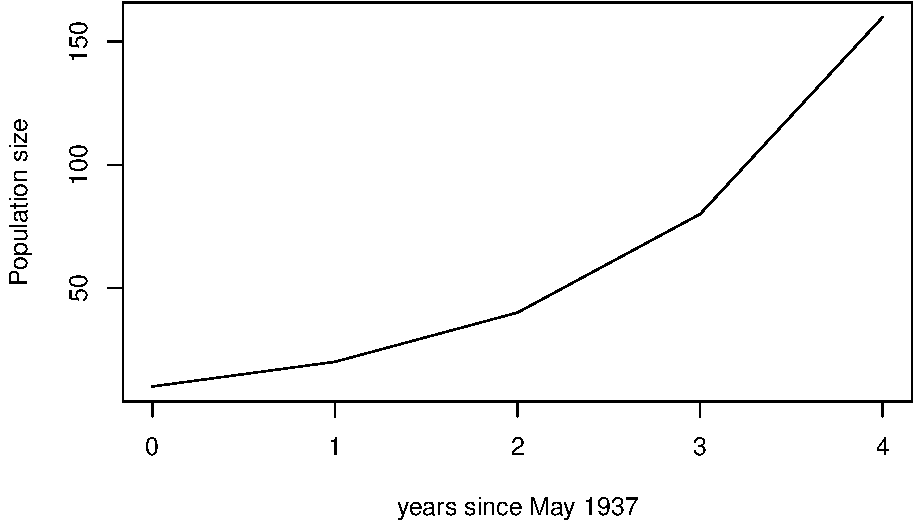
\includegraphics{BIOL-3295_files/figure-latex/unnamed-chunk-18-1.pdf}

If you already have an existing plot you can add new lines using
\texttt{lines()}. For example,

\begin{Shaded}
\begin{Highlighting}[]
\KeywordTok{plot}\NormalTok{(}\KeywordTok{seq}\NormalTok{(}\DecValTok{1}\NormalTok{,}\DecValTok{4}\NormalTok{), }\KeywordTok{c}\NormalTok{(}\DecValTok{1}\NormalTok{,}\DecValTok{3}\NormalTok{,}\DecValTok{4}\NormalTok{,}\DecValTok{2}\NormalTok{), }\DataTypeTok{ylab =} \StringTok{"y-axis"}\NormalTok{, }\DataTypeTok{xlab =} \StringTok{"x-axis"}\NormalTok{)}
\KeywordTok{lines}\NormalTok{(}\KeywordTok{seq}\NormalTok{(}\DecValTok{1}\NormalTok{,}\DecValTok{4}\NormalTok{), }\KeywordTok{seq}\NormalTok{(}\DecValTok{1}\NormalTok{,}\DecValTok{4}\NormalTok{))}
\end{Highlighting}
\end{Shaded}

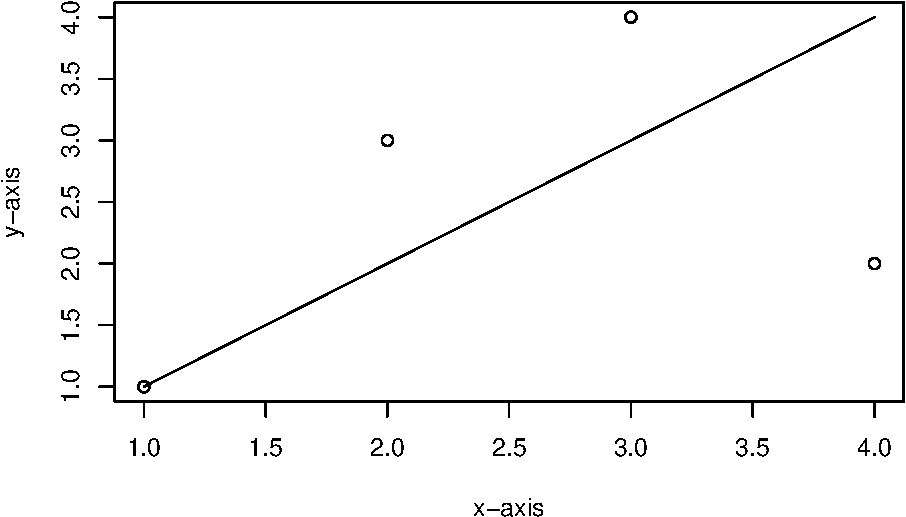
\includegraphics{BIOL-3295_files/figure-latex/unnamed-chunk-19-1.pdf}

 HAND IN

\begin{enumerate}
\def\labelenumi{\arabic{enumi}.}
\setcounter{enumi}{4}
\tightlist
\item
  Write an R scipt that builds on the file you have previously made
  \emph{protection-island.R}. Use the \texttt{lines()} command to add
  the predicted population size assuming geometric growth using the
  commands described in this section. If you have written the code
  correctly the result should look something like this:
\end{enumerate}

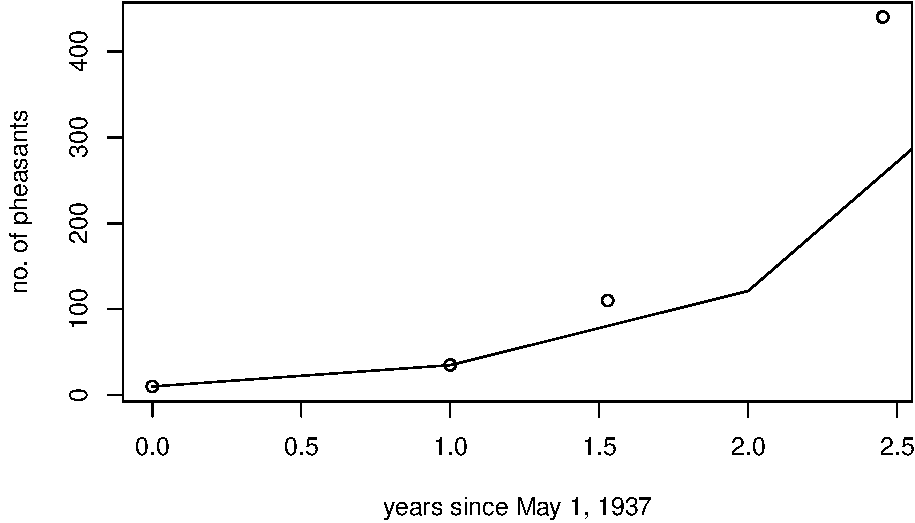
\includegraphics{BIOL-3295_files/figure-latex/unnamed-chunk-20-1.pdf}

Note that to get years on the x-axis for data from the
\emph{protection-island.R} file, I needed to plot \texttt{plot(x/365,y)}
because with \texttt{plot(x,y)} the units on my x-axis were days. Your
graph may look slightly different since you may have calculated a
slightly different \(\lambda\) value if you made different assumptions
to me in questions 1 and 2.

You are to hand in your R Script. See \ref{RScript} for more
information. {[}10 marks{]}

\chapter{Fri Sept 25: Exponential growth (continuous
time)}\label{fri-sept-25-exponential-growth-continuous-time}

DUE DATE: Tues Oct 6

\section{Required reading}\label{required-reading}

Vandermeer, J.H., Goldberg, D.E., 2013. Population Ecology: First
Principles (Second Edition). Princeton University Press, Princeton,
United States. p4-8.
\href{https://ebookcentral-proquest-com.qe2a-proxy.mun.ca/lib/mun/detail.action?docID=1205619}{Link}

We now have two ways of describing how population size changes with time
whereby each individual has the same average number of offspring per
unit time and the same probability of dying.

\begin{enumerate}
\def\labelenumi{\arabic{enumi})}
\tightlist
\item
  Discrete time geometric growth:
\end{enumerate}

\begin{equation}
N_t = N_0\lambda^t
\label{eq:Geo}
\end{equation}

and,

\begin{enumerate}
\def\labelenumi{\arabic{enumi})}
\setcounter{enumi}{1}
\tightlist
\item
  Continuous time exponential growth:
\end{enumerate}

\begin{equation}
N(t) = N(0)e^{rt}
\label{eq:Exp}
\end{equation}

Notably, for both these models the per capita birth and death rates do
not change change over time, and do not change with density or age.

The notation \(N_t\) and \(N(t)\) is conventional for discrete time
versus continuous time formulations respectively, however, these
notations both mean the same: the population size at a particular time,
\(t\). When \(t=0\) we have the population size at time 0: \(N_0\) or
\(N(0)\).

\section{Discrete or continuous time
formulations}\label{discrete-or-continuous-time-formulations}

Whether it is appropriate to model a population in a discrete time or
continous time formulation depends on whether births and deaths are
overlapping or neatly partitioned into a distinct time period. For
example, for many animals there is a distinct breeding season: a short
proportion of the year when offspring are born. As such, there is very
little temporal overlap between the times of year when births and deaths
occur. Humans are an example of a species that might reasonably be
modelled as continuous time because babies are born year round.

\section{Questions}\label{questions}

Please submit the answer to these questions to brightspace, ideally for
the next class, but you have until Sept 30 to complete them without
penalty.

\begin{enumerate}
\def\labelenumi{\arabic{enumi}.}
\item
  In equation \eqref{eq:Exp}, what is \(e\)? {[}1 mark{]}
\item
  For what values of \(r\) does the population size increase over time?
  {[}1 mark{]}
\item
  As described in the reading, \(b\) is a per capita birth rate, and
  \(d\) is a per capita death rate. For continuous time exponential
  growth, both \(b\) and \(d\) must be non-negative and can take values
  bigger than 1. Note that this differs from the discrete time model
  formulation where \(0 \leq d \leq 1\). When \(d > 1\) in the
  continuous time formulation, this means that the average lifespan is
  less than one time step. For example, when \(d = 2\) this means that
  the average life expectancy for an individual is 1/2 a time step
  (i.e., days or year, however, the time unit is defined in the model).
  When the population size increases over time, what is true of \(b\)
  relative to \(d\)? {[}1 mark{]}
\item
  For what value of \(r\) does \(N(t)\) not change over time? Hint: if
  \(N(t)\) is not changing then \(N(t)=N(0)\) for all \(t\). {[}1
  mark{]}
\item
  Consider the equation: \[
  \frac{dN(t)}{dt} = rN(t).
  \] As described in the reading, this is an alternative way to write
  the continuous time exponential growth equation. The quantity
  \(\frac{dN(t)}{dt}\) can be understood as the slope of a graph where
  population size is on the vertical axis and time is on the horizontal
  axis. As such, if the slope is zero, \(\frac{dN(t)}{dt}=0\), then the
  population size is not changing. If \(\frac{dN(t)}{dt}<0\), then the
  population size is decreasing. For what value of \(r\) does the
  population size decrease? What is true about \(b\) relative to \(d\)
  in this instance? {[}2 marks{]}
\item
  Which population would be more appropriate to be modelled as a
  continuous time formulation: \emph{E. coli} bacteria or moose? {[}1
  mark{]}
\item
  Calculate the formula for the doubling time for continuous time
  exponential growth (equation \eqref{eq:Exp}). This is the time for the
  population to double in size. The value of \(N(0)\), the population
  size at \(t=0\) doesn't matter as long as it is a positive number.
  When the population has doubled, \(N(t) = 2N(0)\). To answer this
  question you need to find \(t\) such that \(N(t) = 2N(0)\). You may
  need to revisit some rules about working with logarithms to complete
  this question (i.e.~see
  \href{https://en.wikipedia.org/wiki/Logarithm}{here}, specifically the
  \emph{Product, Quotient, Power, and Root} table. Also recall,
  \(Ln(e^x) = x\)). Please show your work. {[}2 marks{]}
\item
  Consider the following plot:

  \begin{figure}
  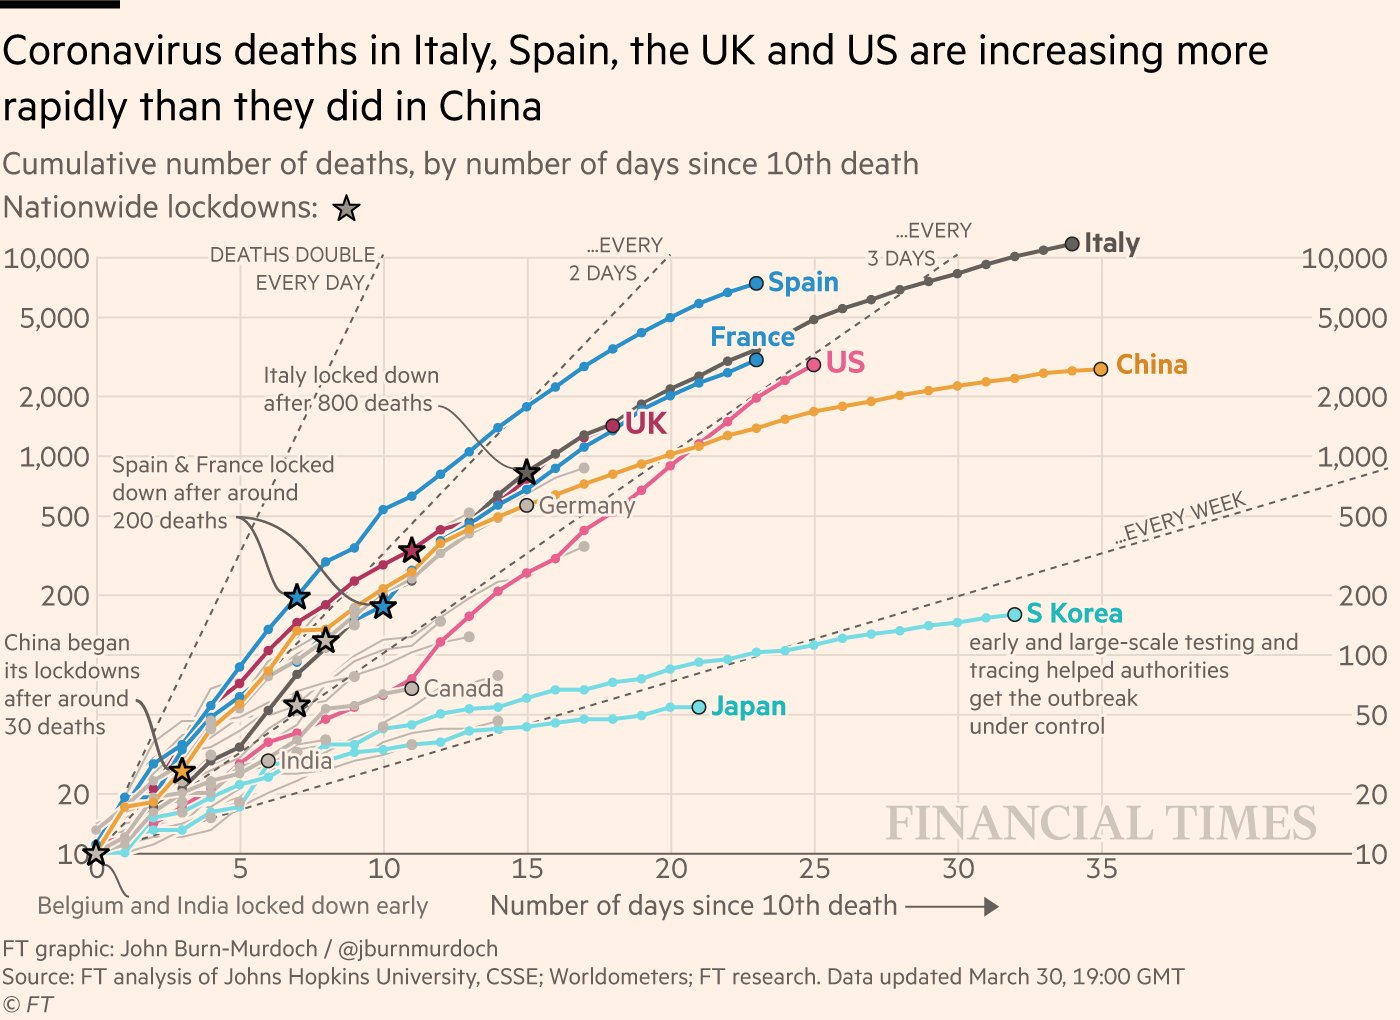
\includegraphics[width=0.95\linewidth]{figures/doublingtime} \caption{An example of a very well thought out data visualation where the data might demonstrate exponential growth}\label{fig:doublingtime}
  \end{figure}
\end{enumerate}

In this question, we will find the equation for `doubles every day'. Our
model is equation \eqref{eq:Exp}. This means that we will calculate the
equation for `doubles every day' under the assumption that cumulative
COVID-19 deaths grow exponentially over time.

To begin, we choose the time step for our model as days. The first
problem we should consider is what is the value of \(r\) if the
population doubles every 1 day? Make the appropriate substitutions and
re-arrange equation \eqref{eq:Exp} to find the value of \(r\).

Now, note that the y-axis on the above graph is on a logarithmic scale.
We will assume this is a base \(e\) logarithmic scale. Take the natural
logarithm of both sides of equation \eqref{eq:Exp}. Note that the result
should be the formula for a straight line, i.e., \(y = mx + c\), but
where \(y\) is \(Ln(N(t))\) and \(x\) is \(t\) (to match the axes of
Figure \ref{fig:doublingtime}). The questions we are left to solve are:
what is the slope of the line (i.e., \(m\), or the value of the
coefficient that multiplies \(t\)), and what is the value of the
intercept (i.e., \(c\) or the remaining terms on the opposite side of
the equals to \(Ln(N(t))\) and which are not multiplied by \(t\))?

Show all your work. Your answer is complete when you provide the
numerical values of the slope and the intercept for the straight line
corresponding to a doubling time of 1 day. Assume \(N(0)=10\). Your
answers must be numbers - you will need to substitute the value of \(r\)
that you calculated in the early part of this question. {[}2 marks{]}

\begin{enumerate}
\def\labelenumi{\arabic{enumi}.}
\setcounter{enumi}{8}
\tightlist
\item
  Provide the values of the slope and the intercept for doubling times
  of 2, 3, and 7 days. Again assume \(N(0)=10\). You do not need to show
  your work. {[}2 marks{]}
\end{enumerate}

\chapter{Tues Sept 29: Doubling time}\label{tues-sept-29-doubling-time}

DUE DATE: Thurs Oct 8

Today we will make a graph of the current COVID-19 data for Ontario.
When only a small fraction of the population is resistant to an
infection, the number of daily cases, in absence of any interventions
such as physical distancing, is expected to grow exponentially over
time. At the end of this exercise you will have calculated the doubling
time for the second wave of COVID-19 in Ontario.

Visit the website: \url{https://art-bd.shinyapps.io/covid19canada/},
this site is the \emph{front end} for the data we will use which are
archived \href{https://github.com/ishaberry/Covid19Canada}{here} (also
referred to as the \emph{back end}). These data can easily be pulled
into \texttt{R} using this command:

\begin{Shaded}
\begin{Highlighting}[]
\NormalTok{COVID.data <-}\StringTok{ }\NormalTok{data.table::}\KeywordTok{fread}\NormalTok{(}\StringTok{'https://raw.githubusercontent.com/ishaberry/Covid19Canada/master/timeseries_prov/active_timeseries_prov.csv'}\NormalTok{, }\DataTypeTok{fill =} \OtherTok{TRUE}\NormalTok{)}
\end{Highlighting}
\end{Shaded}

However, first you will need to install the \texttt{data.table} package:

\begin{Shaded}
\begin{Highlighting}[]
\KeywordTok{install.packages}\NormalTok{(}\StringTok{"data.table"}\NormalTok{)}
\end{Highlighting}
\end{Shaded}

When asked: \emph{Do you want to install from sources the package which
needs compilation? (Yes/no/cancel)} enter \texttt{no}.

To view the data type:

\begin{Shaded}
\begin{Highlighting}[]
\KeywordTok{head}\NormalTok{(COVID.data)}
\end{Highlighting}
\end{Shaded}

\begin{verbatim}
##    province date_active cumulative_cases cumulative_recovered cumulative_deaths
## 1:  Alberta  25-01-2020                0                    0                 0
## 2:  Alberta  26-01-2020                0                    0                 0
## 3:  Alberta  27-01-2020                0                    0                 0
## 4:  Alberta  28-01-2020                0                    0                 0
## 5:  Alberta  29-01-2020                0                    0                 0
## 6:  Alberta  30-01-2020                0                    0                 0
##    active_cases active_cases_change
## 1:            0                   0
## 2:            0                   0
## 3:            0                   0
## 4:            0                   0
## 5:            0                   0
## 6:            0                   0
\end{verbatim}

\texttt{head()} is a command that shows the first 6 lines of the
quantity inside the round brackets. \texttt{COVID.data} is a very large
table of data. If I type \texttt{COVID.data} into the Console I will get
more information than I want, so I instead use \texttt{head()}.

So far we have pulled data from an online repository. However, it is
good practice to save these data in case later the repository is
removed. We can make copy of the data for our records using the
following commands:

Note that the above contains the path to folders on my computer and
saves \texttt{COVID.data} as the file \emph{COVID-data-save.csv}. You
will need to replace the path above with correct path to the folder on
your own computer where you want to save these data. Setting the path is
computer-specific, and so we always have problems with this in class
because the solutions vary by student. Some tricks that work for me are:

\begin{itemize}
\item
  type \texttt{getwd()} into the Console. This will tell you the current
  working directory and can give you clues on the format of the path for
  your computer.
\item
  clicking the \texttt{Source} button on a .R file that you have made
  will print the path to that .R file into the Console.
\item
  elect to save the file somewhere very simple, for example, on your
  Desktop and then move it to a more organized place later.
\end{itemize}

Navigate to the folder where you expected to save the data as a .csv
file. You should be able to open the .csv file in \emph{Microsoft
Excel}. {[}THIS PART DOESN'T WORK - SORRY - JUST SKIP{]}

Now, the data table \texttt{COVID.data} contains data for all provinces
and we would like to \emph{subset} the data so that only the information
pertaining to Ontario is left. We do this as follows:

\begin{Shaded}
\begin{Highlighting}[]
\NormalTok{data.ON <-}\StringTok{ }\NormalTok{COVID.data[province ==}\StringTok{ "Ontario"}\NormalTok{]}
\end{Highlighting}
\end{Shaded}

We should understand what variables are contained in our data set. Query
the following in your Console:

\begin{Shaded}
\begin{Highlighting}[]
\KeywordTok{colnames}\NormalTok{(data.ON)}
\end{Highlighting}
\end{Shaded}

We will plot confirmed positive cases over time:

\begin{Shaded}
\begin{Highlighting}[]
\KeywordTok{plot}\NormalTok{(data.ON$cumulative_cases, }\DataTypeTok{ylab =} \StringTok{"Cumulative cases"}\NormalTok{, }\DataTypeTok{typ =} \StringTok{"l"}\NormalTok{)}
\end{Highlighting}
\end{Shaded}

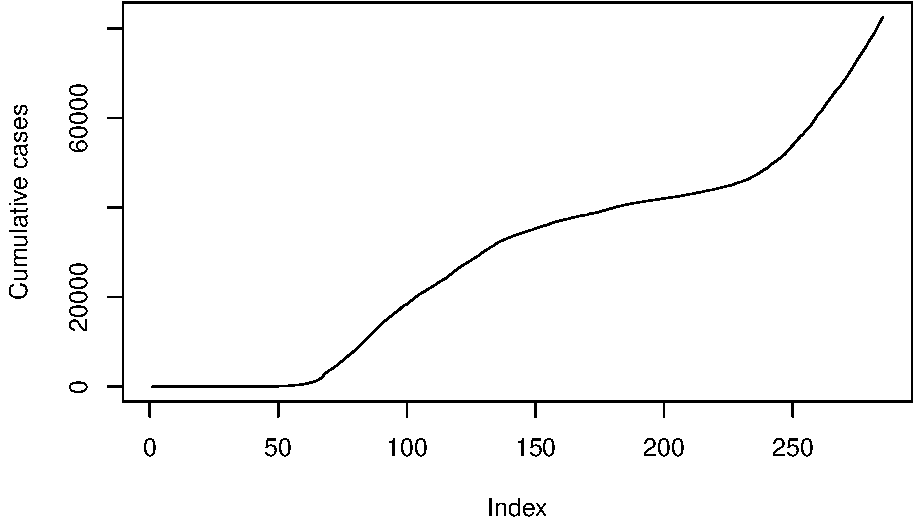
\includegraphics{BIOL-3295_files/figure-latex/unnamed-chunk-27-1.pdf}

Note that we haven't provided an x-axis argument above. The x-axis
should be \texttt{date\_active}, however, from our previous exercise
(Chapter \ref{PE2}), we recognize that dates need to be reformatted to
be an appropriate x-axis.

\begin{Shaded}
\begin{Highlighting}[]
\KeywordTok{head}\NormalTok{(data.ON$date_active)}
\end{Highlighting}
\end{Shaded}

\begin{verbatim}
## [1] "25-01-2020" "26-01-2020" "27-01-2020" "28-01-2020" "29-01-2020"
## [6] "30-01-2020"
\end{verbatim}

The earliest date is January 25, 2020. We will use this as the origin
and calculate the number of days since that time.

\begin{Shaded}
\begin{Highlighting}[]
\KeywordTok{require}\NormalTok{(chron)}
\NormalTok{days.since <-}\StringTok{ }\KeywordTok{julian}\NormalTok{(}\KeywordTok{as.Date}\NormalTok{(data.ON$date_active, }\DataTypeTok{format =} \StringTok{"%d-%m-%Y"}\NormalTok{),}\DataTypeTok{origin=}\KeywordTok{as.Date}\NormalTok{(}\StringTok{"25-01-2020"}\NormalTok{, }\DataTypeTok{format =} \StringTok{"%d-%m-%Y"}\NormalTok{))}
\end{Highlighting}
\end{Shaded}

If you get an error this may be because you have not installed the
\texttt{chron} package. You can do so as
\texttt{install.packages("chron")}.

On my first attempt at the above code, I tried
\texttt{julian(data.ON\$date\_active)}. This generated an error because
our dates from the COVID-19 dataset are formatted as a character string
``01-25-2020'', but the \texttt{julian()} function is expecting three
numerical arguments \texttt{julian(m,d,y)}. As such,
\texttt{julian(data.ON\$Date}) fails to provide three numerical
arguments to the function and instead provides a single character
string. For this reason the function \texttt{as.Date()} needs to be
applied to \texttt{data.ON\$Date} inside the \texttt{julian()} function.

We now have a quantity \texttt{days.since} that is appropriate for the
x-axis of our graph:

\begin{Shaded}
\begin{Highlighting}[]
\KeywordTok{plot}\NormalTok{(days.since, data.ON$cumulative_cases, }\DataTypeTok{ylab =} \StringTok{"cumulative cases"}\NormalTok{, }\DataTypeTok{xlab =} \StringTok{"days since Jan 25, 2020"}\NormalTok{, }\DataTypeTok{typ =} \StringTok{"l"}\NormalTok{)}
\end{Highlighting}
\end{Shaded}

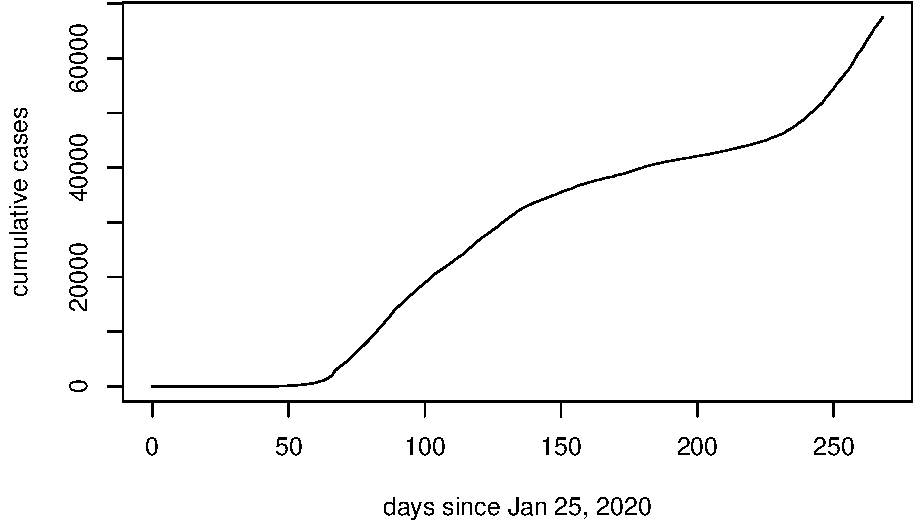
\includegraphics{BIOL-3295_files/figure-latex/unnamed-chunk-30-1.pdf}

However, rather than calculating cumumlative cases suppose that we might
like to plot daily new cases. We do this by subtracting the cumulative
cases for the previous day. The function \texttt{diff()} subtracts the
element previous to the entry of a list and because the first element of
the list has not preceeding value we add in a 0.

\begin{Shaded}
\begin{Highlighting}[]
\NormalTok{new.cases <-}\StringTok{ }\KeywordTok{diff}\NormalTok{(}\KeywordTok{c}\NormalTok{(}\DecValTok{0}\NormalTok{,data.ON$cumulative_cases))}
\KeywordTok{plot}\NormalTok{(days.since, new.cases, }\DataTypeTok{ylab =} \StringTok{"new cases"}\NormalTok{, }\DataTypeTok{xlab =} \StringTok{"days since Jan 25, 2020"}\NormalTok{, }\DataTypeTok{typ =} \StringTok{"l"}\NormalTok{)}
\end{Highlighting}
\end{Shaded}

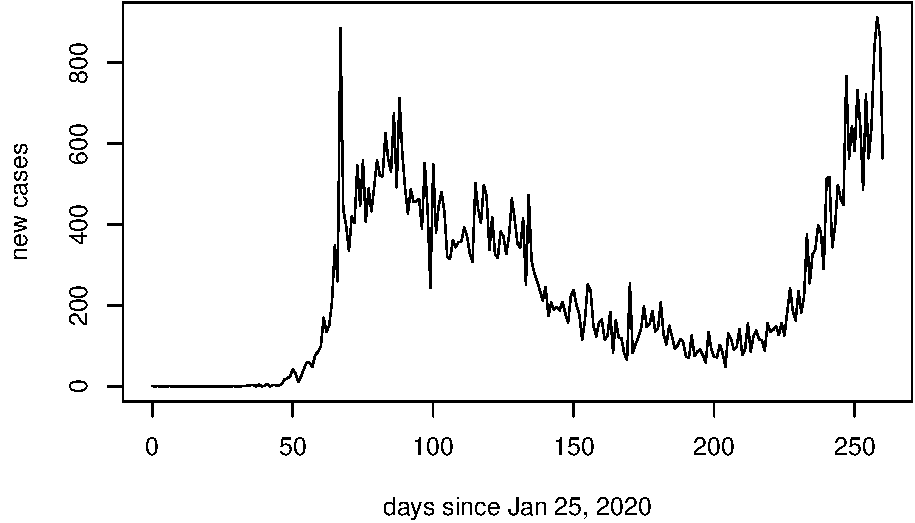
\includegraphics{BIOL-3295_files/figure-latex/unnamed-chunk-31-1.pdf}

If we have done a good job of our work, it should be consistent with the
official graph labelled as (B) below:

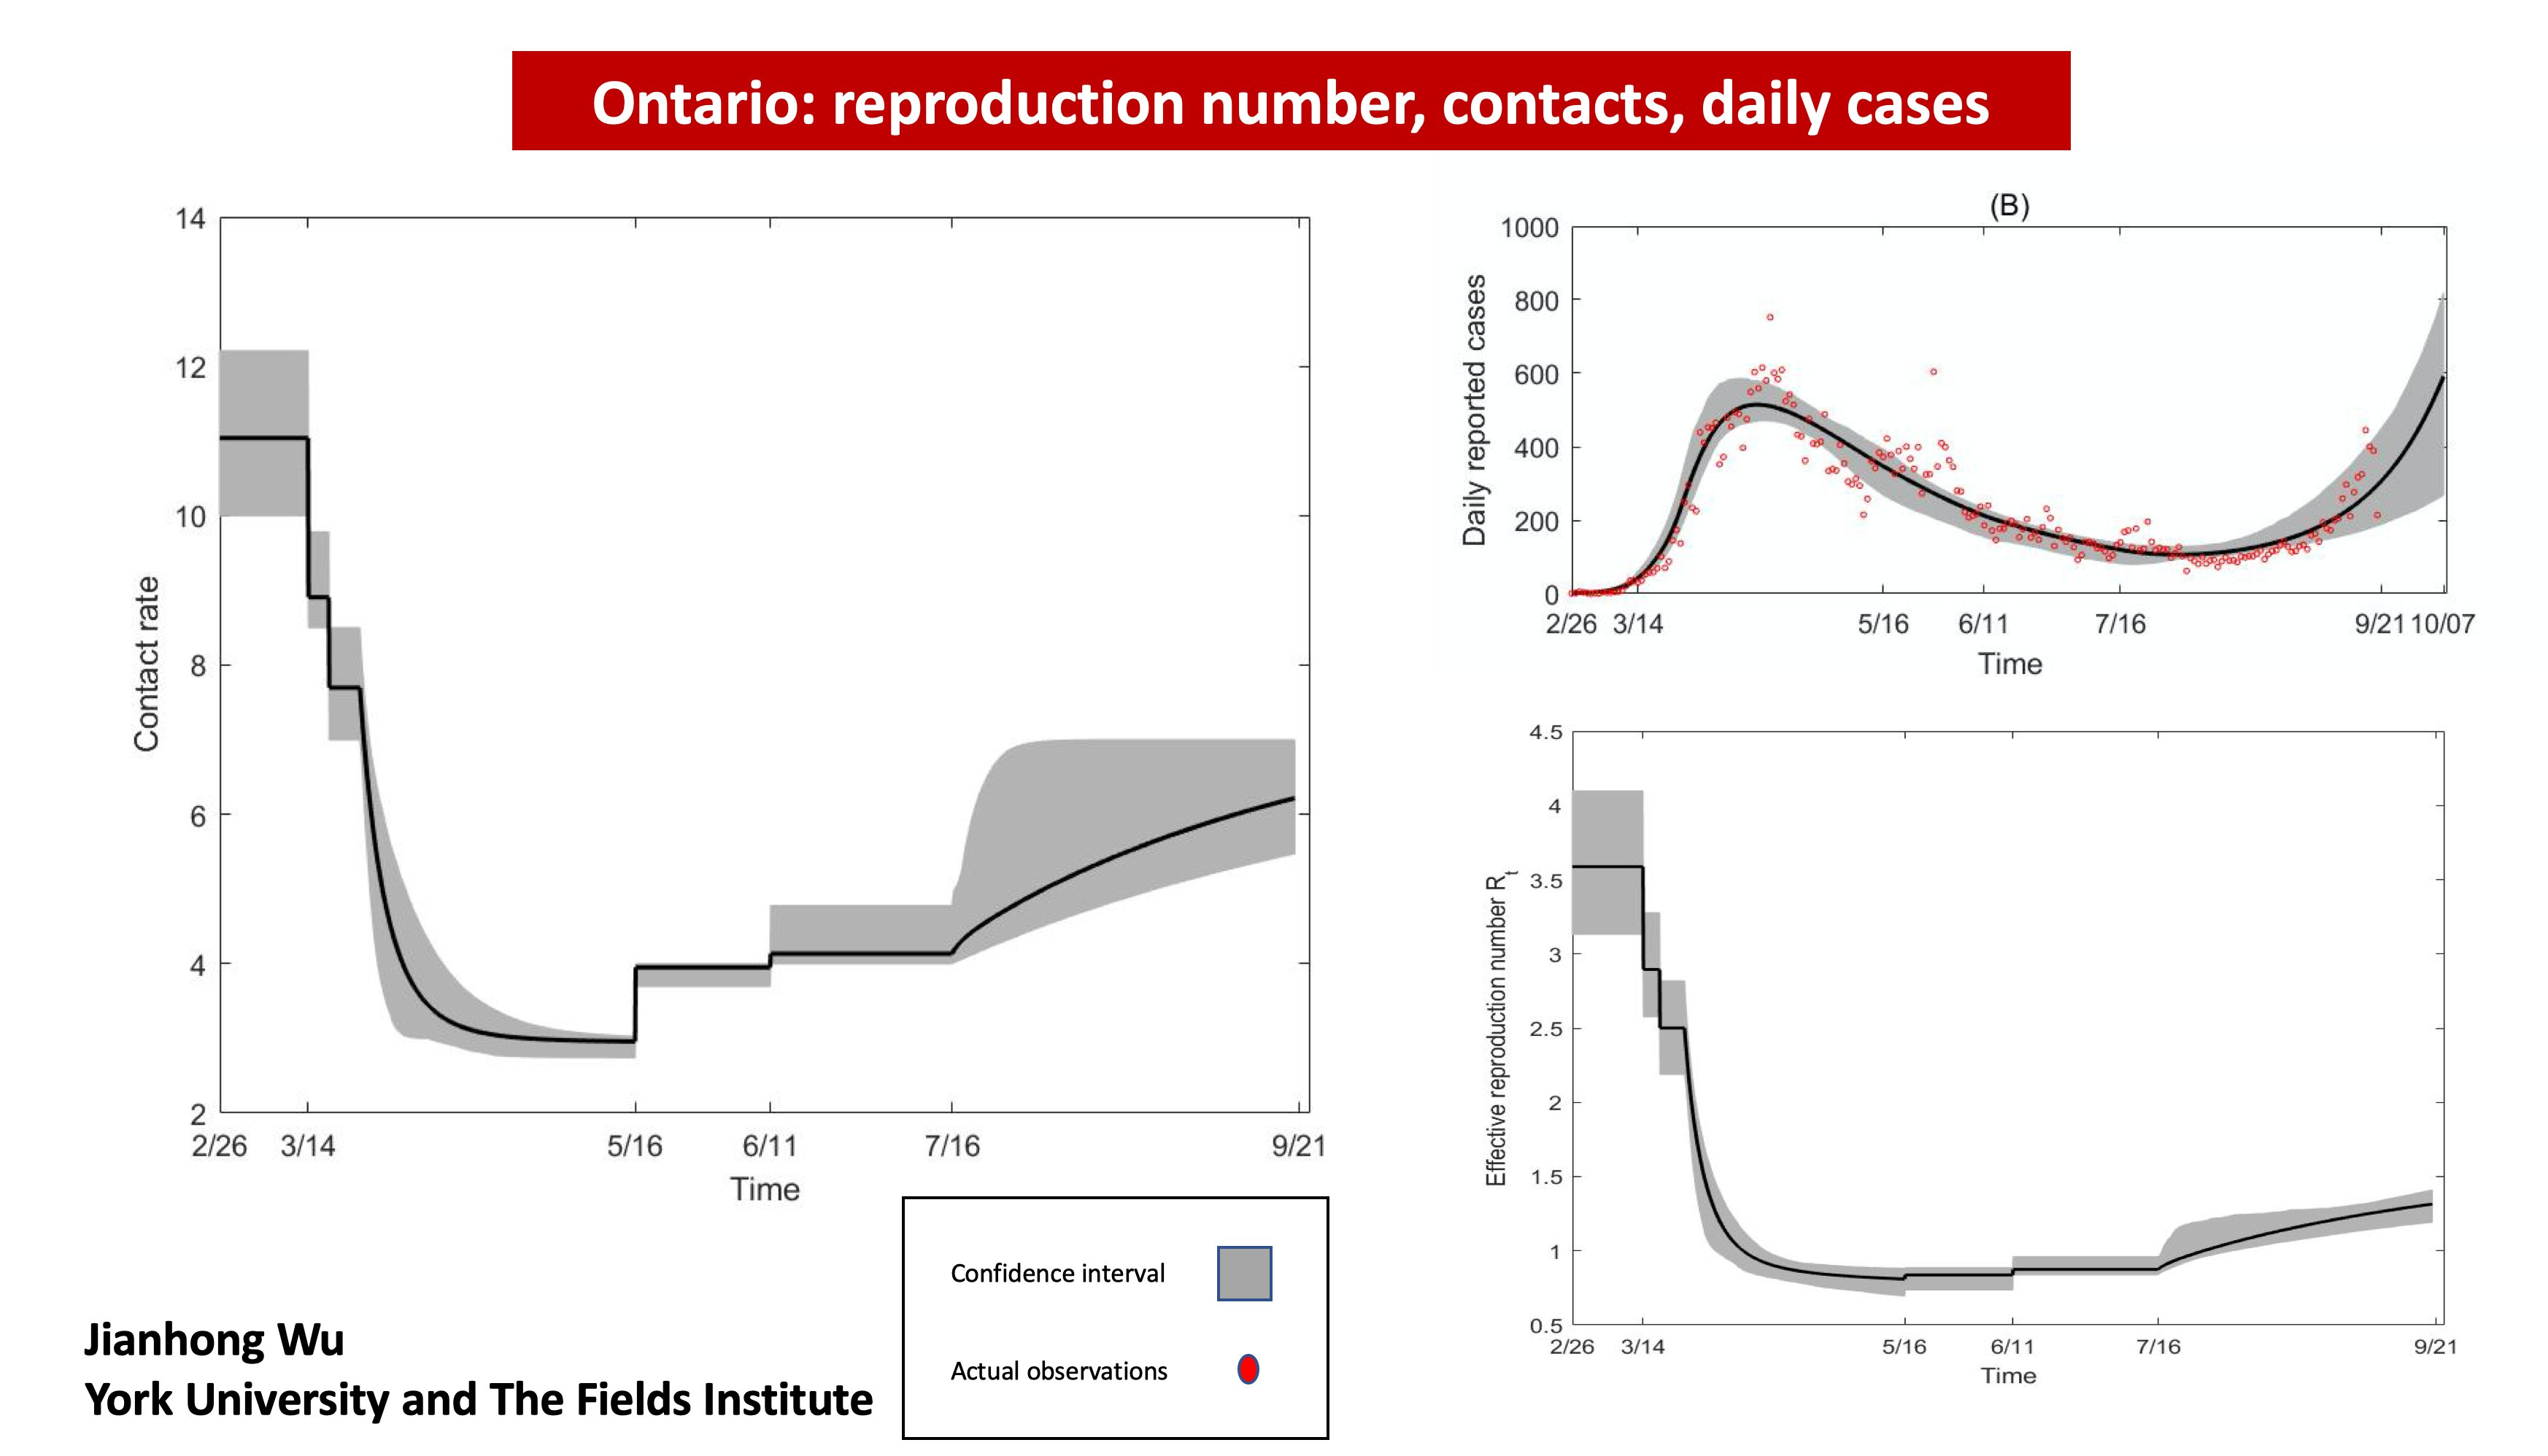
\includegraphics[width=1.2\linewidth]{figures/ONData}

We can also focus in on just the second wave by adjusting the
\texttt{xlim} argument:

\begin{Shaded}
\begin{Highlighting}[]
\KeywordTok{plot}\NormalTok{(days.since[}\DecValTok{200}\NormalTok{:}\KeywordTok{max}\NormalTok{(days.since)], new.cases[}\DecValTok{200}\NormalTok{:}\KeywordTok{max}\NormalTok{(days.since)], }\DataTypeTok{ylab =} \StringTok{"new cases"}\NormalTok{, }\DataTypeTok{xlab =} \StringTok{"days since Jan 25, 2020"}\NormalTok{, }\DataTypeTok{pch =} \DecValTok{16}\NormalTok{)}
\end{Highlighting}
\end{Shaded}

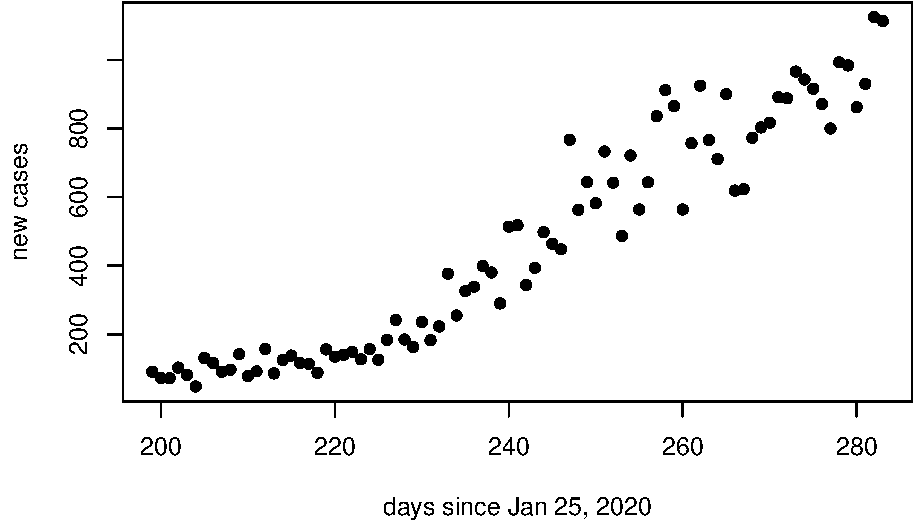
\includegraphics{BIOL-3295_files/figure-latex/unnamed-chunk-32-1.pdf}

Note that the second wave of COVID-19 in Ontario appears to be
consistent with exponential growth. Recall that when the y-axis of the
graph is on a logarithmic scale, exponential growth will be represented
as a straight line.

\begin{figure}
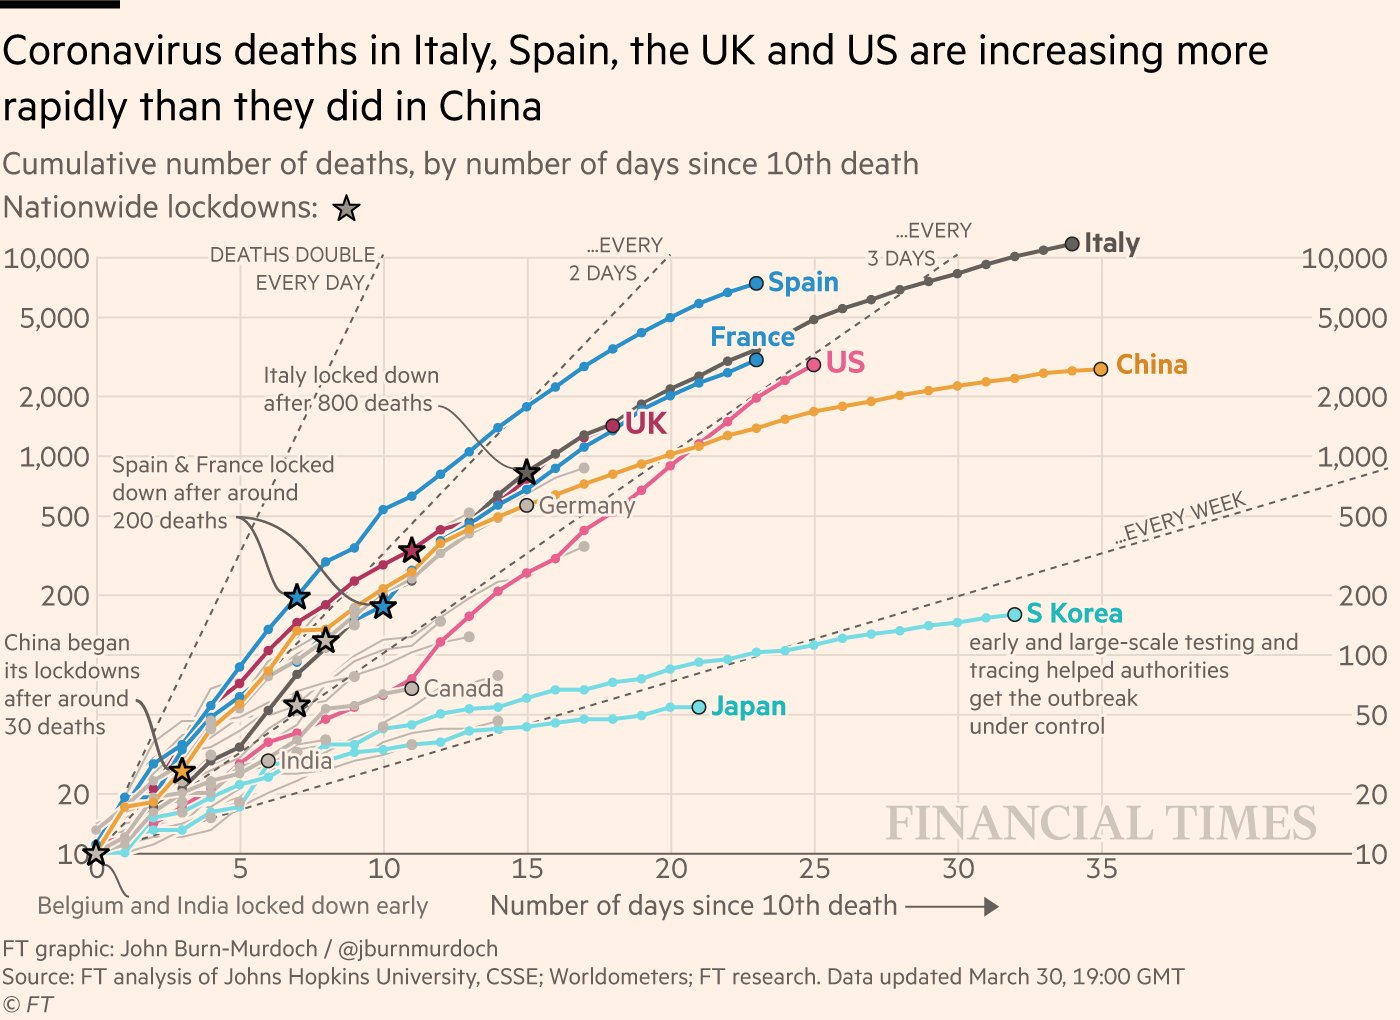
\includegraphics[width=0.95\linewidth]{figures/doublingtime} \caption{Straight lines illustrate exponential growth with different doubling times when the y-axis is plotted on a logarithmic scale}\label{fig:doublingtime2}
\end{figure}

We can estimate the doubling time of the number of new cases for the
second wave of COVID-19 in Ontario by perfoming a linear regression on
the natural logarithm of the number of new cases. Below, we consider
only the data 224 days after January 25 and onwards. The function
\texttt{lm()} performs the linear regression and \texttt{abline()} plots
the regression.

\begin{Shaded}
\begin{Highlighting}[]
\NormalTok{since}\FloatTok{.225} \NormalTok{<-}\StringTok{ }\NormalTok{days.since[}\DecValTok{225}\NormalTok{:}\KeywordTok{max}\NormalTok{(days.since)]}
\NormalTok{log.cases}\FloatTok{.225} \NormalTok{<-}\StringTok{ }\KeywordTok{log}\NormalTok{(new.cases[}\DecValTok{225}\NormalTok{:}\KeywordTok{max}\NormalTok{(days.since)])}
\KeywordTok{plot}\NormalTok{(since}\FloatTok{.225}\NormalTok{,log.cases}\FloatTok{.225}\NormalTok{, }\DataTypeTok{ylab =} \StringTok{"log(new cases)"}\NormalTok{, }\DataTypeTok{xlab =} \StringTok{"days since Jan 25, 2020"}\NormalTok{, }\DataTypeTok{pch =} \DecValTok{16}\NormalTok{)}
\NormalTok{reg <-}\StringTok{ }\KeywordTok{lm}\NormalTok{(log.cases}\FloatTok{.225}\NormalTok{~since}\FloatTok{.225}\NormalTok{)}
\KeywordTok{abline}\NormalTok{(reg)}
\end{Highlighting}
\end{Shaded}

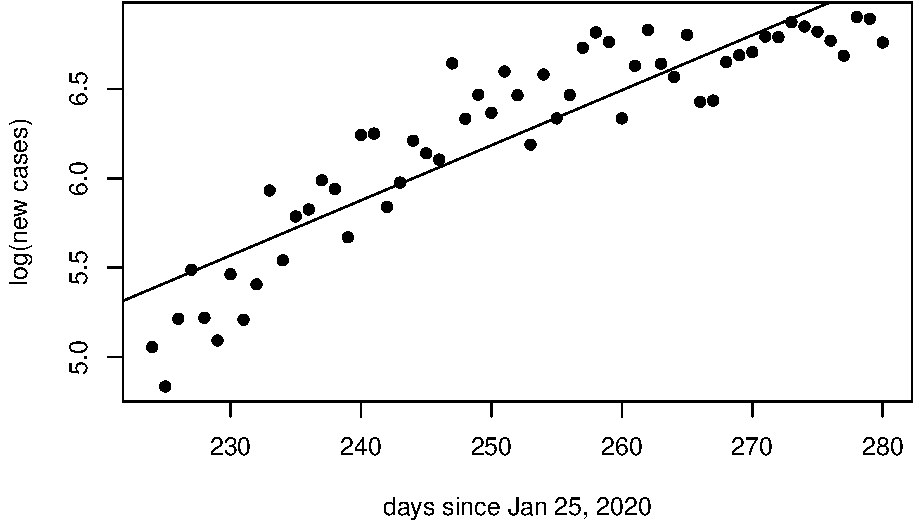
\includegraphics{BIOL-3295_files/figure-latex/unnamed-chunk-33-1.pdf}

\begin{Shaded}
\begin{Highlighting}[]
\KeywordTok{summary}\NormalTok{(reg)}
\end{Highlighting}
\end{Shaded}

\begin{verbatim}
## 
## Call:
## lm(formula = log.cases.225 ~ since.225)
## 
## Residuals:
##      Min       1Q   Median       3Q      Max 
## -0.60429 -0.16363 -0.01929  0.19167  0.55580 
## 
## Coefficients:
##              Estimate Std. Error t value Pr(>|t|)    
## (Intercept) -1.167490   0.448929  -2.601   0.0117 *  
## since.225    0.029369   0.001763  16.657   <2e-16 ***
## ---
## Signif. codes:  0 '***' 0.001 '**' 0.01 '*' 0.05 '.' 0.1 ' ' 1
## 
## Residual standard error: 0.2425 on 59 degrees of freedom
## Multiple R-squared:  0.8246, Adjusted R-squared:  0.8217 
## F-statistic: 277.4 on 1 and 59 DF,  p-value: < 2.2e-16
\end{verbatim}

From the summary of the linear regression we are interested in the
slope, because in the previous class we estimated the relationship
between this slope and the doubling time.

\begin{figure}
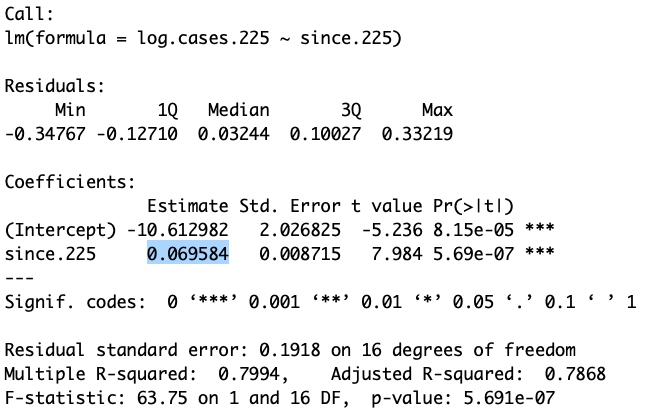
\includegraphics[width=0.95\linewidth]{figures/regression} \caption{The above output shows the slope of the regression as 0.0695 log cases per day}\label{fig:regression}
\end{figure}

\section{Questions}\label{questions}

\begin{enumerate}
\def\labelenumi{\arabic{enumi}.}
\item
  How many observations and how many variables are there in the
  \texttt{COVID.data} and the \texttt{data.ON} files? (see the
  \emph{Environment} tab) {[}1 mark{]}
\item
  What command did you use to save the data as a .csv file? - IGNORE
  THIS QUESTION - INSTRUCTIONS WERE BAD {[}1 mark{]}
\item
  What do you estimate the doubling time of the second wave of COVID-19
  in Ontario to be? Show your calculations {[}3 marks{]}
\item
  Write an R Script that performs the linear regression as illustrated
  above. Your script must make the figure including the regression line
  {[}7 marks{]}
\end{enumerate}

\chapter{Thurs Oct 1: Density dependence and logistic
growth}\label{thurs-oct-1-density-dependence-and-logistic-growth}

DUE DATE: Friday Oct 9

\section{Required reading}\label{required-reading}

Vandermeer, J.H., Goldberg, D.E., 2013. Population Ecology: First
Principles (Second Edition). Princeton University Press, Princeton,
United States. p9-17.
\href{https://ebookcentral-proquest-com.qe2a-proxy.mun.ca/lib/mun/detail.action?docID=1205619}{Link}

\section{Questions}\label{questions}

\begin{enumerate}
\def\labelenumi{\arabic{enumi}.}
\item
  What is the equation for continous time logistic growth in its
  \emph{classic form}? Define all the symbols in the equation by writing
  their meanings in words. Can \(K\) be negative? {[}3 marks{]}
\item
  What does dN/dt mean? {[}1 mark{]}
\item
  Assume that \(N < K\). For what values of \(r\) will \(N\) increase
  over time? {[}1 mark{]}
\item
  Assume that \(r > 0\) and \(K > N\). Will \(N\) increase or decrease
  in size over time? {[}1 mark{]}
\item
  Assume that \(r,K \neq 0\). For what values of \(N\) is the population
  size constant (i.e., not changing over time)? {[}2 marks{]}
\item
  What is the main difference between exponential and logistic growth?
  {[}1 mark{]}
\end{enumerate}

\chapter{Tues Oct 6: Solving the logistic growth equation using a
computer 1}\label{NumSolve1}

ANNOUNCEMENT: Friday Oct 2 is a catch-up day

DUE DATE: Tues Oct 13

Recall that for continous time exponential growth there were two ways
that the equation might be written. Firstly, as a \emph{change} in
population size over time,

\begin{equation}
\frac{dN(t)}{dt} = rN(t),
\label{eq:Exp1}
\end{equation}

such that if \(\frac{dN(t)}{dt}>0\), the population size, \(N(t)\) is
increasing over time, and if \(\frac{dN(t)}{dt}<0\), the population size
is decreasing over time. Alternatively, we can write continuous time
exponential growth as,

\begin{equation}
N(t) = N(0)e^{rt},
\label{eq:Exp2}
\end{equation}

where the lefthand side of equation \eqref{eq:Exp2} states the \emph{size}
of the population, \(N(t)\), at time \(t\), rather than the
\emph{change} in the size of the population, as it did in equation
\eqref{eq:Exp1}.

For logistic growth, we have:

\begin{equation}
\frac{dN(t)}{dt} = rN(t)\left(1 - \frac{N(t)}{K} \right).
\label{eq:Log1}
\end{equation}

How might we find the equivalent of equation \eqref{eq:Exp2} for logistic
growth? i.e., for logistic growth, what is the equation for the
\emph{size} of the population at a particular time, \(t\)? If you are
great at math, you might integrate equation \eqref{eq:Log1} using
\href{https://math.usu.edu/~powell/ysa-html/node8.html}{separation of
variables}. However, another option, that we will build towards for next
class, is to numerically integrate equation \eqref{eq:Log1} using a
computer.

\section{What is an ordinary differential
equation?}\label{what-is-an-ordinary-differential-equation}

In an introductory calculus course that covers integration, most often
you are solving problems of the type:

\begin{eqnarray}
\frac{dy(x)}{dx} &=& x^2, \\
\int \frac{dy(x)}{dx} &=& \int x^2 \ dx, \\
y(x) &=& \frac{1}{3}x^3 + c.
\label{eq:e1}
\end{eqnarray}

Note that in the above calculations, we are able to use integration to
find \(y(x)\) when we are given the rate of change equation,
\(\frac{dy(x)}{dx}\). In the above equations, \(x\), is the independent
variable, \(y(x)\) is the dependent variable, the derivative of \(y(x)\)
is with respect to \(x\), and \(x\) appears on the opposite side of the
\texttt{=} to the derivative of the dependent variable. In the notation
of population biology, where \(N(t)\) is conventional for the dependent
variable, a similar problem might look like this:

\begin{eqnarray}
\int \frac{dN(t)}{dt} &=& \int rt \ dt, \\ \nonumber
N(t) &=& \frac{1}{2}rt^2 + c. 
\label{eq:e2}
\end{eqnarray}

We have not seen any equations like equation \eqref{eq:e2} in BIOL 3295 so
far: usually, our equations for the \emph{change} in the population
size, \(\frac{dN(t)}{dt}\), have a dependency on the population size,
\(N(t)\) (the dependent variable), rather than a sole dependency on
\(t\) (the independent variable).

The equations that are models for population biology are sometimes ODEs.
While some ODEs can be solved using math, commonly the ODEs that are
used to model population dynamics need to be integrated numerically;
that is, using a computer.

\section{Numerically integrating an ordinary differential equation in
R}\label{numerically-integrating-an-ordinary-differential-equation-in-r}

Numerical integration in \texttt{R} can be performed by installing this
package:

\begin{Shaded}
\begin{Highlighting}[]
\KeywordTok{install.packages}\NormalTok{(}\StringTok{"deSolve"}\NormalTok{)}
\end{Highlighting}
\end{Shaded}

To integrate our ODE, we use the function \texttt{ode()} from the
\texttt{deSolve} package. Let's look at the structure of this function.
The mandatory arguments to the function are:

\texttt{ode(y,times,parms,func)}

where,

\texttt{y} is a vector of the initial values of the dependent variable
(i.e., those which correspond to the initial time).

\texttt{times} is a sequence of time points that we will calculate the
values of the variables; the first value of times is the initial time.

\texttt{func} is a function that computes the values of the derivatives
of the dependent variables. \texttt{func} must be defined as:
\texttt{func\ \textless{}-\ function(t,\ y,\ parms,...)}. \texttt{t} is
the current time point in the integration, and \texttt{y} is the current
estimate of the variables in the ODE system.

Given what we have learned in BIOL 3295 so far, \texttt{y} and
\texttt{times} are not so tricky, but the \texttt{func} arguement
requires us to write our own function, and so far we have only used
functions written by other people: we have yet to write our own custom
functions. In preparation for next class, when we will numerically
integrate the logistic growth equation, we will next learn how to write
custom functions.

\section{Writing custom functions}\label{writing-custom-functions}

Generally, your code can still work without writing custom functions,
however writing functions makes your code modular and more organized.

Consider the following code:

\begin{Shaded}
\begin{Highlighting}[]
\CommentTok{# Temperatures in Celcius}
\NormalTok{temp.min.C <-}\StringTok{ }\DecValTok{10}
\NormalTok{temp.max.C <-}\StringTok{ }\DecValTok{20}

\CommentTok{# Temperatures in Farenheit}
\NormalTok{temp.min.F <-}\StringTok{ }\NormalTok{temp.min.C*}\DecValTok{9}\NormalTok{/}\DecValTok{5+32}
\NormalTok{temp.max.F <-}\StringTok{ }\NormalTok{temp.max.C*}\DecValTok{9}\NormalTok{/}\DecValTok{5+32} 
\end{Highlighting}
\end{Shaded}

The above code is fine, but since the same calculation is performed
twice (conversion of Celcius to Farenheit), just with a different
number, we might consider writing a custom function. Let's re-write the
above code so that it now uses a custom function:

\begin{Shaded}
\begin{Highlighting}[]
\CommentTok{# A function that converts Celcius to Farenheit}
\NormalTok{C.to.F <-}\StringTok{ }\NormalTok{function(C)\{}
  \NormalTok{F <-}\StringTok{ }\NormalTok{C*}\DecValTok{9}\NormalTok{/}\DecValTok{5} \NormalTok{+}\DecValTok{32}
  \KeywordTok{return}\NormalTok{(F)}
\NormalTok{\}}

\CommentTok{# Temperatures in Celcius}
\NormalTok{temp.min.C <-}\StringTok{ }\DecValTok{10}
\NormalTok{temp.max.C <-}\StringTok{ }\DecValTok{20}

\CommentTok{# Temperatures in Farenheit}
\NormalTok{temp.min.F <-}\StringTok{ }\KeywordTok{C.to.F}\NormalTok{(temp.min.C)}
\NormalTok{temp.max.F <-}\StringTok{ }\KeywordTok{C.to.F}\NormalTok{(temp.max.C)}
\end{Highlighting}
\end{Shaded}

Note that the above code consists of the \emph{function definition} and
the \emph{function call}. The function definition uses the function
\texttt{function()}.

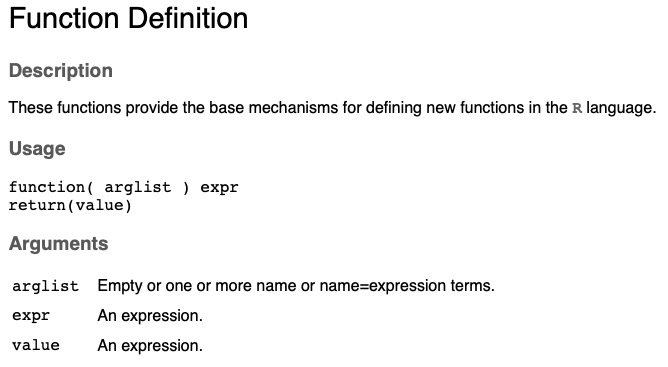
\includegraphics[width=1.2\linewidth]{figures/function}

In the example, note the following:

\begin{itemize}
\item
  \texttt{arglist} is just one value: \texttt{C}. Generally, several
  values might be provided to the function where each should be
  separated by commas and enclosed within the \texttt{()}.
\item
  \texttt{expression} can be any set of commands and should be enclosed
  within the \texttt{\{\}}.
\item
  The function is assigned a name: \texttt{C.to.F}. We give the function
  a name so that we can use it later during a function call.
\end{itemize}

\section{Questions}\label{questions}

\begin{enumerate}
\def\labelenumi{\arabic{enumi}.}
\tightlist
\item
  The following is an equation for exponential population growth with a
  constant immigration rate, \(m>0\), into the population:
\end{enumerate}

\[
\frac{dN(t)}{dt}= rN(t) + m
\]

where \(r\) is the net reproductive rate, and \(N(t)\) is the population
size at time, \(t\).

Is this equation an ordinary differential equation (ODE)? Give 1
sentence explaining your reasoning {[}2 marks{]}.

\begin{enumerate}
\def\labelenumi{\arabic{enumi}.}
\setcounter{enumi}{1}
\tightlist
\item
  Write a function that adds 123 to a user supplied argument, and then
  write the line of code that calls the function to evaluate 123+1, and
  assigns the result the variable name \texttt{y}. You are to hand in
  your R script. {[}5 marks{]}
\end{enumerate}

\chapter{Thurs Oct 8: Solving the logistic growth equation using a
computer 2}\label{NumSolve2}

DUE DATE: Thursday Oct 15

Last class we learned how to make a custom function. Today we would like
to write a custom function that satisfies the requirements of the
\texttt{func} argument that is supplied to \texttt{ode()} so that
numerical integration can be performed.

\section{Writing the func argument for
ode()}\label{writing-the-func-argument-for-ode}

The \texttt{func} argument of \texttt{ode()} has the following
constraints:

\begin{itemize}
\tightlist
\item
  The \texttt{arglist} must include \texttt{t}, \texttt{y}, and
  \texttt{parms}.
\item
  The value returned must be a \emph{list} of the rates of change in the
  dependent variable(s).
\end{itemize}

Note that if your ODE comprises of more than one variable that is
changing over time, then \texttt{y} will be a vector. Below is an
example of how \texttt{func} might be coded for exponential growth.
Remember that the ODE for exponential growth is:

\begin{equation}
\frac{dN(t)}{dt} = rN(t) 
\label{eq:Exp99}
\end{equation}

Below equation \eqref{eq:Exp99} is coded in the appropriate syntax for
eventual use in the \texttt{ode()} function:

\begin{Shaded}
\begin{Highlighting}[]
\CommentTok{# Write a function that returns a list of the rate of change in your dependent variables.}
\NormalTok{model =}\StringTok{ }\NormalTok{function(t,y,parms)\{}
  \CommentTok{# It's a personal perference of mine to switch the symbols}
  \CommentTok{# to be consistent with the equation.}
  \NormalTok{N <-}\StringTok{ }\NormalTok{y[}\DecValTok{1}\NormalTok{]}
  \CommentTok{# This is this equation for dN/dt}
  \NormalTok{dN <-}\StringTok{ }\NormalTok{r*N}
  \CommentTok{# The function returns the value of the change in N.}
\KeywordTok{return}\NormalTok{(}\KeywordTok{list}\NormalTok{(}\KeywordTok{c}\NormalTok{(dN)))}
\NormalTok{\}}
\end{Highlighting}
\end{Shaded}

Let's try out the function to make sure it works. Copy and paste the
function into your \texttt{Console} and then type:

\begin{Shaded}
\begin{Highlighting}[]
\NormalTok{r<-}\DecValTok{1}
\KeywordTok{model}\NormalTok{(}\DecValTok{1}\NormalTok{,}\DecValTok{2}\NormalTok{,}\DataTypeTok{parms=}\OtherTok{NULL}\NormalTok{)}
\end{Highlighting}
\end{Shaded}

Did you get \texttt{2}? Does it make sense to you that the returned
value is \texttt{2}? Try some other values. Are the values making sense?

Now that the \texttt{func} argument of \texttt{ode()} has been
demonstrated, the remaining arguments for the \texttt{ode()} function
are not so bad.

\begin{Shaded}
\begin{Highlighting}[]
\CommentTok{# The initial value of N}
\NormalTok{yini<-}\StringTok{ }\KeywordTok{c}\NormalTok{(}\DataTypeTok{N =} \DecValTok{1}\NormalTok{)}

\CommentTok{# the times for the numerical integration}
\NormalTok{times <-}\StringTok{ }\KeywordTok{seq}\NormalTok{(}\DecValTok{0}\NormalTok{, }\DecValTok{1}\NormalTok{, }\DataTypeTok{by =} \NormalTok{.}\DecValTok{1}\NormalTok{)}
\end{Highlighting}
\end{Shaded}

Rembember to assign a value for \texttt{r}:

\begin{Shaded}
\begin{Highlighting}[]
\CommentTok{# Asign a value to the parameter:}
\NormalTok{r <-}\StringTok{ }\DecValTok{2}
\end{Highlighting}
\end{Shaded}

And then once all the arguments are set, call the function, and plot the
results:

\begin{Shaded}
\begin{Highlighting}[]
\CommentTok{# performing the numerical integration}
\NormalTok{out <-}\StringTok{ }\KeywordTok{ode}\NormalTok{(}\DataTypeTok{y =} \NormalTok{yini, }\DataTypeTok{parms =} \OtherTok{NULL}\NormalTok{, }\DataTypeTok{times =} \NormalTok{times, }\DataTypeTok{func =} \NormalTok{model)}
\NormalTok{out <-}\StringTok{ }\KeywordTok{data.frame}\NormalTok{(out)}
\KeywordTok{head}\NormalTok{(out)}

\CommentTok{# this line overrides a multipanel plot. I had tried plot(out) # and was having conflicts with a small plotting window on my}
\CommentTok{# laptop. Generally, the below line isn't necessary.}
\KeywordTok{par}\NormalTok{(}\DataTypeTok{mfrow=}\KeywordTok{c}\NormalTok{(}\DecValTok{1}\NormalTok{,}\DecValTok{1}\NormalTok{))}

\CommentTok{# Make the graph}
\KeywordTok{plot}\NormalTok{(out$time, out$N, }\DataTypeTok{typ =} \StringTok{"l"}\NormalTok{)}
\end{Highlighting}
\end{Shaded}

\section{Questions}\label{questions}

\begin{enumerate}
\def\labelenumi{\arabic{enumi}.}
\item
  For the code \texttt{model(1,2,parms=NULL)} (where the function
  \texttt{model} is defined above), what do \texttt{1} and \texttt{2}
  correspond to? One of these quantities does not affect the value that
  the \texttt{model()} function returns. Which quantity does not affect
  the value the function returns? {[}2 marks{]}
\item
  Write an R Script that numerically integrates the logistic growth
  function (equation \eqref{eq:Log1}). Choose a value of \(r\) such that
  the population size increases over time. Remember to use good
  practices for writing your script - see \ref{RScript}. Your script
  should produce a graph with \(N(t)\) on the y-axis and time on the
  x-axis {[}10 marks{]}
\item
  Add to your script from 2. such that another graph is produced, this
  time where the population size decreases over time. Note that this
  should just require adding new lines to the bottom of your question 1
  script such that you: a) set a new value of \texttt{r}; b) run the
  \texttt{ode()} command; and c) make the graph. In other words, it is
  not necessary to define the logistic growth function, \texttt{model},
  again because that has not changed. Further, if you are happy to use
  the same values of \texttt{times} as for question 1, you do not need
  to restate this either. Answer this question by adding a few lines of
  code to your answer to 1. You are to hand in your R script. You should
  answer both questions 1. and 2. in the same R script. {[}5 marks{]}
\end{enumerate}

\chapter{Fri Oct 9 and Thurs Oct 15: Data and the logistic
equation}\label{fri-oct-9-and-thurs-oct-15-data-and-the-logistic-equation}

DUE DATE: Thurs Oct 22

\section{Questions}\label{questions}

\begin{enumerate}
\def\labelenumi{\arabic{enumi}.}
\item
  Question 1.9 on p12 of
  \href{https://ebookcentral-proquest-com.qe2a-proxy.mun.ca/lib/mun/detail.action?docID=1205619}{Vandermeer
  and Gordon} (but completed following the instructions below). Hand-in
  your graph with a figure caption. Your graph should have the intrinsic
  growth rate on the y-axis and population size (in millions) on the
  x-axis. In response to `what kind of function would describe the data
  reasonably well', you just need to answer an increasing or decreasing
  function. {[}10 marks{]}
\item
  Based on your work in question 1, what is the value of the intrinsic
  growth when \(t = 1955, 2013\) and \(2014\)? {[}2 marks{]}
\item
  If a population is growing exponentially, and the intrinsic growth
  rate is plotted on the y-axis, and population size is plotted on the
  x-axis, what is the slope of the line? What does the intercept of the
  graph tell us? {[}2 marks{]}
\end{enumerate}

\section{The data}\label{the-data}

Question 1.9 in Vandermeer and Goldberg involves a large data table. It
will be very boring to have to type all those numbers in by hand.
Fortunately, here is a
\href{https://ourworldindata.org/world-population-growth}{website}, with
a link to a similiar data set. Lets load in the data:

\begin{Shaded}
\begin{Highlighting}[]
\NormalTok{pop.data <-}\StringTok{ }\KeywordTok{read.csv}\NormalTok{(}\StringTok{'https://ourworldindata.org/uploads/2013/05/WorldPopulationAnnual12000years_interpolated_HYDEandUNto2015.csv'}\NormalTok{)}
\end{Highlighting}
\end{Shaded}

Lets take a look at our data by entering the following in the console:

\begin{Shaded}
\begin{Highlighting}[]
\KeywordTok{head}\NormalTok{(pop.data)}
\end{Highlighting}
\end{Shaded}

\begin{verbatim}
##     year World.Population..Spline.Interpolation.until.1950.
## 1 -10000                                            2431214
## 2  -9999                                            2432196
## 3  -9998                                            2433179
## 4  -9997                                            2434162
## 5  -9996                                            2435145
## 6  -9995                                            2436129
\end{verbatim}

Lets find out the column names of our data. Type the following into your
console:

\begin{Shaded}
\begin{Highlighting}[]
\KeywordTok{colnames}\NormalTok{(pop.data)}
\end{Highlighting}
\end{Shaded}

\begin{verbatim}
## [1] "year"                                              
## [2] "World.Population..Spline.Interpolation.until.1950."
\end{verbatim}

The second column name is weird. Let's replace it with a better name:

\begin{Shaded}
\begin{Highlighting}[]
\KeywordTok{colnames}\NormalTok{(pop.data)<-}\KeywordTok{c}\NormalTok{(}\StringTok{"year"}\NormalTok{, }\StringTok{"size"}\NormalTok{)}
\end{Highlighting}
\end{Shaded}

The data we have loaded starts in 10,000 B.C., but the Vandermeer and
Goldberg data just starts in 1955. The code below identifies which rows
correspond to 1955 onwards.

\begin{Shaded}
\begin{Highlighting}[]
\NormalTok{ind <-}\StringTok{ }\KeywordTok{which}\NormalTok{(pop.data$year>=}\DecValTok{1955}\NormalTok{)}
\end{Highlighting}
\end{Shaded}

Let's make a new dataset that only contains the data for 1955 onwards:

\begin{Shaded}
\begin{Highlighting}[]
\NormalTok{pop.data}\FloatTok{.1955} \NormalTok{<-}\StringTok{ }\NormalTok{pop.data[ind,]}
\end{Highlighting}
\end{Shaded}

In the above code the square brackets are the
\texttt{{[}rows,columns{]}} that we are extracting. Note that the rows
we would like, we have assigned the variable name \texttt{ind}. When the
column argument is left blank this is understood to be all columns (or
in this case, \emph{both} columns: \texttt{year} and \texttt{size}).

Let's plot our data, but to make things easier, let's change the
population size into millions (where \texttt{1e6} is scientific notation
for millions).

\begin{Shaded}
\begin{Highlighting}[]
\NormalTok{pop.data}\FloatTok{.1955}\NormalTok{$size <-}\StringTok{ }\NormalTok{pop.data}\FloatTok{.1955}\NormalTok{$size/}\FloatTok{1e6}
\KeywordTok{plot}\NormalTok{(pop.data}\FloatTok{.1955}\NormalTok{$year, pop.data}\FloatTok{.1955}\NormalTok{$size, }\DataTypeTok{typ =} \StringTok{"l"}\NormalTok{, }\DataTypeTok{xlab =} \StringTok{"year"}\NormalTok{, }\DataTypeTok{ylab =} \StringTok{"popn size (in millions)"}\NormalTok{)}
\end{Highlighting}
\end{Shaded}

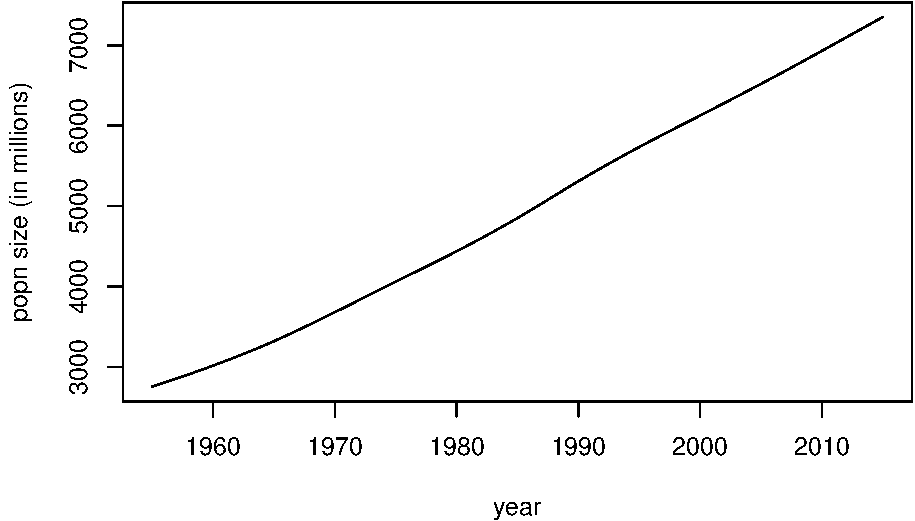
\includegraphics{BIOL-3295_files/figure-latex/unnamed-chunk-48-1.pdf}

\section{The intrinsic growth rate}\label{the-intrinsic-growth-rate}

Now, consider the equation,

\begin{equation}
N_{t+1} = r(N_t)N_t.
\label{eq:R}
\end{equation}

This equation states that the population size in the next time step
(\(N_{t+1}\)) is equal to the population size at time \(t\) (which is
\(N_t\)), multiplied by the intrinsic growth rate, \(r(N_t)\), where the
intrinsic growth rate might depend on population size (which is why
\(r(N_t)\) is written that way: you can read it as `\(r\) is a function
of \(N_t\)'). For example, with exponential growth, the intrinsic growth
rate does not change with population size, so \(r(N_t) = \lambda\).
However, when population growth demonstrates negative density
dependence, then \(r(N_t)\) would be a decreasing function of population
size, \(N_t\).

Consider the Beverton-Holt equation which is equation 28 on p29 of
Vandermeer and Goldberg:

\[
N_{t+1} = \frac{\lambda N_t}{1+\alpha N_t}.
\]

Note that this could be written in the form of equation \eqref{eq:R}
where,

\begin{equation}
r(N_t) = \frac{\lambda}{1+\alpha N_t}.
\end{equation}

Therefore, the Beverton-Holt equation demonstrates negative density
dependence since the intrinsic growth rate, \(r(N_t)\), is a decreasing
function of population size, \(N_t\).

By re-arranging equation \eqref{eq:R}, we can see that the intrinsic
growth rate is calculated as:

\[
r(N_t) = \frac{N_{t+1}}{N_t},
\]

such that the intrinsic growth rate can be understood as a ratio of
population sizes at consecutive time points. How might we calculate the
intrinsic growth rate for our data?

First, we should note that Question 1.9 in Vandermeer and Goldberg asks
us to plot the intrinsic growth rate (y-axis) versus the population size
(x-axis). Let's take \(N_{1955} = 2758\): this is our first x-axis
value, but what is the corresponding y-value? The answer is:

\[
r(N_{1955}) = \frac{N_{1956}}{N_{1955}} = \frac{N_{t+1}}{N_t} \mbox{ where $t = 1955$}.
\]

Note that the numerator values will be the sequence of values

\([N_{1956}, N_{1957}, ..., N_{2015}]\),

and the denomenator values will be the sequence of values

\([N_{1955}, N_{1956}, ..., N_{2014}]\).

Therefore, the numerator values are the list of all population sizes
except the first value (\(N_{1955}\)), and the denomenator values are
the list of all population sizes except the last value (\(N_{2015}\)).
The functions \texttt{head()} and \texttt{tail()} can be used to remove
values from a list:

\begin{Shaded}
\begin{Highlighting}[]
\NormalTok{numerator <-}\StringTok{ }\KeywordTok{tail}\NormalTok{(pop.data}\FloatTok{.1955}\NormalTok{$size,-}\DecValTok{1}\NormalTok{)}
\NormalTok{denomenator <-}\StringTok{ }\KeywordTok{head}\NormalTok{(pop.data}\FloatTok{.1955}\NormalTok{$size,-}\DecValTok{1}\NormalTok{)}
\end{Highlighting}
\end{Shaded}

And then we can calculate the list of intrinsic growth rates,
\(r(N_t)\):

\begin{Shaded}
\begin{Highlighting}[]
\NormalTok{r <-}\StringTok{ }\NormalTok{numerator/denomenator}
\end{Highlighting}
\end{Shaded}

Now consider the values we need for our x-axis. The last value of
\(r(N_t)\) that we calculated was
\(\frac{N_{2015}}{N_{2014}} = \frac{N_{t+1}}{N_t}\) when \(t=2014\),
which means that the last value of \(N_t\) we have a corresponding
\(r(N_t)\) value for is \(N_{2014}\). Therefore, our x-axis nees to be:

\begin{Shaded}
\begin{Highlighting}[]
\NormalTok{Nt <-}\StringTok{ }\KeywordTok{head}\NormalTok{(pop.data}\FloatTok{.1955}\NormalTok{$size,-}\DecValTok{1}\NormalTok{)}
\end{Highlighting}
\end{Shaded}

Finally, we need to make the plot as required by Question 1.9.

\begin{Shaded}
\begin{Highlighting}[]
\KeywordTok{plot}\NormalTok{(Nt, r, }\DataTypeTok{typ =} \StringTok{"l"}\NormalTok{)}
\end{Highlighting}
\end{Shaded}

It will be your job to put appropriate axes labels on the plot.

\section{References}\label{references}

Vandermeer, J.H., Goldberg, D.E., 2013. Population Ecology: First
Principles (Second Edition). Princeton University Press, Princeton,
United States.
\href{https://ebookcentral-proquest-com.qe2a-proxy.mun.ca/lib/mun/detail.action?docID=1205619}{Link}

\chapter{Tues Oct 20: Density-yield and the discrete time density
dependence}\label{tues-oct-20-density-yield-and-the-discrete-time-density-dependence}

DUE DATE: Tues Oct 27

\section{Required reading}\label{required-reading}

Vandermeer, J.H., Goldberg, D.E., 2013. Population Ecology: First
Principles (Second Edition). Princeton University Press, Princeton,
United States. p17-19 and 28-29.
\href{https://ebookcentral-proquest-com.qe2a-proxy.mun.ca/lib/mun/detail.action?docID=1205619}{Link}

\section{Questions}\label{questions}

\begin{enumerate}
\def\labelenumi{\arabic{enumi}.}
\item
  Logistic growth assumes density dependence in the population growth
  rate. This, however, may be insufficient in many applications. In the
  section, \emph{The Yield-Density Relationship} what solution is
  proprosed? {[}2 marks{]}
\item
  As written in Vandermeer and Gordon the Shinozaki-Kira equation is
  presented without an \texttt{=}. Write the complete equation, by
  adding in an equals and quantity on the other size of the equals.
  Define all the parameters and variables in the equation. {[}2 marks{]}
\item
  The Beverton-Holt equation is equation (28) on p29. There are two
  values of \(N_t\) such that \(N_t = N_{t+1}\). One value can be found
  by re-arranging,
\end{enumerate}

\[
1 = \frac{\lambda}{1+\alpha N_t},
\]

until \(N_t\) is isolated on one side. To find the other value inspect
the equation,

\[
N_{t+1} = \frac{\lambda N_t}{1+\alpha N_t}.
\]

What is another value of \(N_t\) such that \(N_{t+1}=N_t\) {[}4
marks{]}.

\chapter{Thurs Oct 22: Introduction to age-structured population
dynamics}\label{thurs-oct-22-introduction-to-age-structured-population-dynamics}

DUE DATE: Oct 29

\section{Required Reading}\label{required-reading}

Vandermeer, J.H., Goldberg, D.E., 2013. Population Ecology: First
Principles (Second Edition). Princeton University Press, Princeton,
United States. p30-31.
\href{https://ebookcentral-proquest-com.qe2a-proxy.mun.ca/lib/mun/detail.action?docID=1205619}{Link}

The reading mentions \emph{`readers who have forgotten their linear
algebra'}, however, linear algebra is not a pre-requisite for BIOL 3295.
To learn enough linear algebra to complete today's questions you might
watch this 4 minute
\href{https://www.youtube.com/watch?v=Awcj447pYuk}{video} explaining how
to multiply a matrix by a column vector on the right.

We are learning a little bit of linear algebra now because the notation
is compact and because later this formulation will be helpful to
calculate the year-to-year multiplicative change in the population size.

Let's consider an age-structured population where:

\begin{itemize}
\item
  Individuals aged less than 1 year old do not reproduce, and will
  survive to 1 year old with a probability of 0.5.
\item
  Individuals aged less than 2 years old have 2 offspring and then die.
\end{itemize}

We can write the equations for the number of individuals in each stage
one year from now as:

\begin{eqnarray}
N_{1,t+1} & = & 2 N_{2,t}, \nonumber \\
N_{2,t+1} & = & 0.5 N_{1,t}, 
 \label{eq:N1N2}
\end{eqnarray}

where \(N_{1,t+1}\) is the number of individuals aged less than 1 year
at time \(t+1\), and \(N_{2,t+1}\) is the number of individuals aged
between 1 and 2 years at time \(t+1\). Try out the system of equations:
suppose, \(N_{1,0} = 10\) and \(N_{2,0} = 5\), what is \(N_{1,1}\) and
\(N_{2,1}\)?

Note that in the system of equations \eqref{eq:N1N2}, some of the values
that were zeros were omitted, i.e.,

\begin{eqnarray}
N_{1,t+1} & = & 0 N_{1,t} + 2 N_{2,t}, \nonumber \\
N_{2,t+1} & = & 0.5 N_{1,t} + 0 N_{2,t},
 \label{eq:ver2}
\end{eqnarray}

Note that as written above, consistency with the ordering is necessary:
\(N_{1,t+1}\) appears above \(N_{2,t+1}\), and on the other side of the
\texttt{=} \(N_{1,t}\) always appears to the left of \(N_{2,t}\). When
written as the system of equations \eqref{eq:ver2}, we can now more easily
write the system of equations \eqref{eq:N1N2} in matrix notation:

\begin{equation}
\left[
\begin{array}{c}
N_{1,t+1}\\
N_{2,t+1}\\
\end{array}
\right]
=
\left[
\begin{array}{cc}
0 & 2\\
0.5 & 0\\
\end{array}
\right]
\left[
\begin{array}{c}
N_{1,t}\\
N_{2,t}\\
\end{array}
\right]
\label{eq:ver3}
\end{equation}

Again, let \(N_{1,0} = 10\) and \(N_{2,0} = 5\). Using the system of
equations \eqref{eq:ver3}, and remembering how to
\href{https://www.youtube.com/watch?v=Awcj447pYuk}{multiply a matrix by
a column vector}, what is \(N_{1,1}\) and \(N_{2,1}\)? Did you get the
same answer (but now formatted as a vector) as you did to this same
question, but when the problem wasn't in matrix notation (i.e., equation
\eqref{eq:N1N2})? Yes? Super!

Now, we have two equivalent ways to write our population models with age
structure. This may seem unhelpful now, but remember that later matrix
notation will be helpful to calculate the rate of population increase
and the ratio of individuals in the age or stage classes.

\section{Questions}\label{questions}

\begin{enumerate}
\def\labelenumi{\arabic{enumi}.}
\tightlist
\item
  Consider an age-structured population where:
\end{enumerate}

\begin{itemize}
\item
  Individuals aged less than 1 year old do not reproduce, and will
  survive to 1 year old with a probability of 0.2.
\item
  Individuals aged less than 2 years old have 4 offspring and then die.
\end{itemize}

Write the equations for the number of indviduals in each age class in
one year from now, in the format of the system of equations
\eqref{eq:N1N2} {[}2 marks{]}

\begin{enumerate}
\def\labelenumi{\arabic{enumi}.}
\setcounter{enumi}{1}
\item
  Using your system of equations from question 1, assume that at \(t=0\)
  there are 4 individuals aged less than 1 year, and 4 individuals aged
  1 to 2 years. Calculate the number of individuals in each of the two
  age classes at \(t=1\). {[}1 mark{]}
\item
  Following from question 2, the total population size at \(t=1\) can be
  calculated by summing the number of individuals in each of the age
  classes. What is the total number of individuals in the population at
  time \(t=1\)? {[}1 mark{]}
\item
  Re-write your equations from question 1 in matrix notation as
  demonstrated in equation \eqref{eq:ver3}. {[}2 marks{]}
\item
  Using your system of equations from question 4, assume that at \(t=0\)
  there are 2 individuals aged less than 1 year, and 10 individuals aged
  1 to 2 years. Calculate the number of individuals in each of the two
  age classes at \(t=1\). Show your calculations. {[}2 marks{]}
\end{enumerate}

\chapter{Fri Oct 23: Stage-structured population
dynamics}\label{fri-oct-23-stage-structured-population-dynamics}

DUE DATE: Oct 30

Some great visuals
\href{https://twitter.com/seb_schreiber/status/1318574271854116866}{here}
from Dr.~Sebastian Schreiber.

\section{Required Reading}\label{required-reading}

Vandermeer, J.H., Goldberg, D.E., 2013. Population Ecology: First
Principles (Second Edition). Princeton University Press, Princeton,
United States. p39-40.
\href{https://ebookcentral-proquest-com.qe2a-proxy.mun.ca/lib/mun/detail.action?docID=1205619}{Link}

Where \(\mathbb{P}\) is a projection matrix, the element \(p_{ij}\) is
the contribution \emph{from} individuals in stage \(j\) at time \(t\),
\emph{to} stage \(i\) at time \(t+1\),

\begin{equation}
\mathbb{P} = 
\left[
\begin{array}{ccccc}
p_{11} & p_{12} & \dots & \dots & p_{1n} \\
p_{21} & p_{22} & \dots & \dots & p_{2n} \\
\vdots & \vdots & \vdots & \vdots & \vdots \\
p_{n1} & \dots & \dots & \dots & p_{nn} \\
\end{array}
\right].
\end{equation}

Note that it is convention for both age-structured and stage-structured
population models that the most immature stages: i.e, newborns, eggs, or
offspring are indexed as \(i,j = 1\), and progressively more mature
stages are indexed with progressively larger indexes. For example, in
Question 3 below the sensible choice of indexes is:

\(i,j = 1:\) larvae

\(i,j = 2:\) pupae

\(i,j = 3:\) adults

\section{Questions}\label{questions}

\begin{enumerate}
\def\labelenumi{\arabic{enumi}.}
\item
  Consider the projection matrix of the age-structured model from the
  previous class:

  \begin{equation}
  \left[
  \begin{array}{cc}
  0 & 2\\
  0.5 & 0\\
  \end{array}
  \right]
  \end{equation}

  What are the special characteristics of the projection matrix for an
  age-structured population model (Leslie-Lewis matrix), that don't
  necessarily occur for a stage-structured population model (Leftkovitch
  matrix)? {[}1 mark{]}
\item
  Which elements of the Leftkovitch matrix may be larger than 1? Note
  that elements of the matrix occurring in a horizontal line are called
  rows, and elements occurring in a vertical line are called columns.
  {[}1 mark{]}
\item
  Complete Exercise 2.15 on p40 of Vandermeer and Goldberg (2013). This
  question is a bit tricky, so here's a hint. The correct answer for the
  projection matrix has this form:
\end{enumerate}

\begin{equation}
\mathbb{P} = 
\left[
\begin{array}{ccc}
p_{11} & p_{12} & 50 \\
p_{21} & p_{22} & p_{23}\\
p_{31} & p_{32} & p_{33}\\
\end{array}
\right].
\end{equation}

Note that it isn't necessary to include eggs as a stage because after a
month either all eggs have become larvae or died.

{[}3 marks{]}.

\chapter{Tues Oct 27: Data for stage-structured population
dynamics}\label{tues-oct-27-data-for-stage-structured-population-dynamics}

DUE DATE: Tues Nov 3

Install and load the package \texttt{popbio}.

\begin{Shaded}
\begin{Highlighting}[]
\KeywordTok{install.packages}\NormalTok{(}\StringTok{"popbio"}\NormalTok{)}
\KeywordTok{require}\NormalTok{(popbio)}
\end{Highlighting}
\end{Shaded}

Click on the \texttt{popbio} package in the Package tab, or click
\href{https://cran.r-project.org/web/packages/popbio/popbio.pdf}{here}

Today, you will explore some of the data that is available through the
\texttt{popbio} package.

\section{Questions}\label{questions}

\begin{enumerate}
\def\labelenumi{\arabic{enumi}.}
\tightlist
\item
  After reading the documentation about the \texttt{popbio} package,
  select one of the datasets. Do not select \emph{Aquilegia chrysantha}
  as this will be used as the example. For the dataset that you have
  selected, give the details of the source of the data, ideally, a
  peer-reviewed publication, or permanent online repository with
  document. For \emph{Aquilegia chrysantha} I did an internet search to
  find a
  \href{https://www.fs.fed.us/rm/pubs/rmrs_p023/rmrs_p023_070_077.pdf}{technical
  report} that nicely describes the \texttt{aq.trans} dataset. For my
  answer to this question I will provide the full citation:
\end{enumerate}

Stubben, Chris J.; Milligan, Brook G. 2001. The demography of a small
population of yellow columbines in the Organ Mountains. In: Maschinski,
Joyce; Holter, Louella, tech. eds. Southwestern rare and endangered
plants: Proceedings of the Third Conference; 2000 September 25-28;
Flagstaff, AZ. Proceedings RMRS-P-23. Fort Collins, CO: U.S. Department
of Agriculture, Forest Service, Rocky Mountain Research Station.
p.~70-77.

and the link:
\url{https://www.fs.fed.us/rm/pubs/rmrs_p023/rmrs_p023_070_077.pdf}

For your dataset you might not be able to find all these details. For
your answer please provide 1 sentence describing your search strategy
and what you found. {[}2 marks{]}

\begin{enumerate}
\def\labelenumi{\arabic{enumi}.}
\setcounter{enumi}{1}
\tightlist
\item
  View your dataset. For \emph{Aquilegia chrysantha} this is completed
  as:
\end{enumerate}

\begin{Shaded}
\begin{Highlighting}[]
\KeywordTok{head}\NormalTok{(aq.trans)}
\end{Highlighting}
\end{Shaded}

List the column headings of your dataset and provide their meaning. {[}2
marks{]} (for some datasets this is a lot of work, for others it's less
work)

\begin{enumerate}
\def\labelenumi{\arabic{enumi}.}
\setcounter{enumi}{2}
\tightlist
\item
  Visit the section of the \texttt{popbio} package description
  describing the \texttt{grizzly} data. Cut and paste the example code
  into an R script. Run the example code and produce the figures. Hand
  in the figure with the title \emph{`Grizzly log population growth
  rates'} with a figure caption (see Section \ref{figures} for
  expectations). Note that \(\log(1)=0\). As an aside, to be consistent
  with the y-axis, the x-axis would better be labelled as \emph{Number
  of females in year \(t\), \(N_t\)}. It is fine to leave this error
  uncorrected. {[}2 marks{]}
\end{enumerate}

\chapter{Thurs Oct 29-Tues Nov 3:
Midterm}\label{thurs-oct-29-tues-nov-3-midterm}

DUE DATE: Fri Nov 6 at 5pm

\section{Chapter 1 in Vandermeer and
Goldberg}\label{chapter-1-in-vandermeer-and-goldberg}

Vandermeer, J.H., Goldberg, D.E., 2013. Population Ecology: First
Principles (Second Edition). Princeton University Press, Princeton,
United States. Chapter 1.
\href{https://ebookcentral-proquest-com.qe2a-proxy.mun.ca/lib/mun/detail.action?docID=1205619}{Link}

Complete the table below by providing a response in all locations where
there is \textbf{a number in a box}. Some of the table has already been
completed to give you an idea of how to answer the questions. {[}20
marks{]}

\begin{figure}
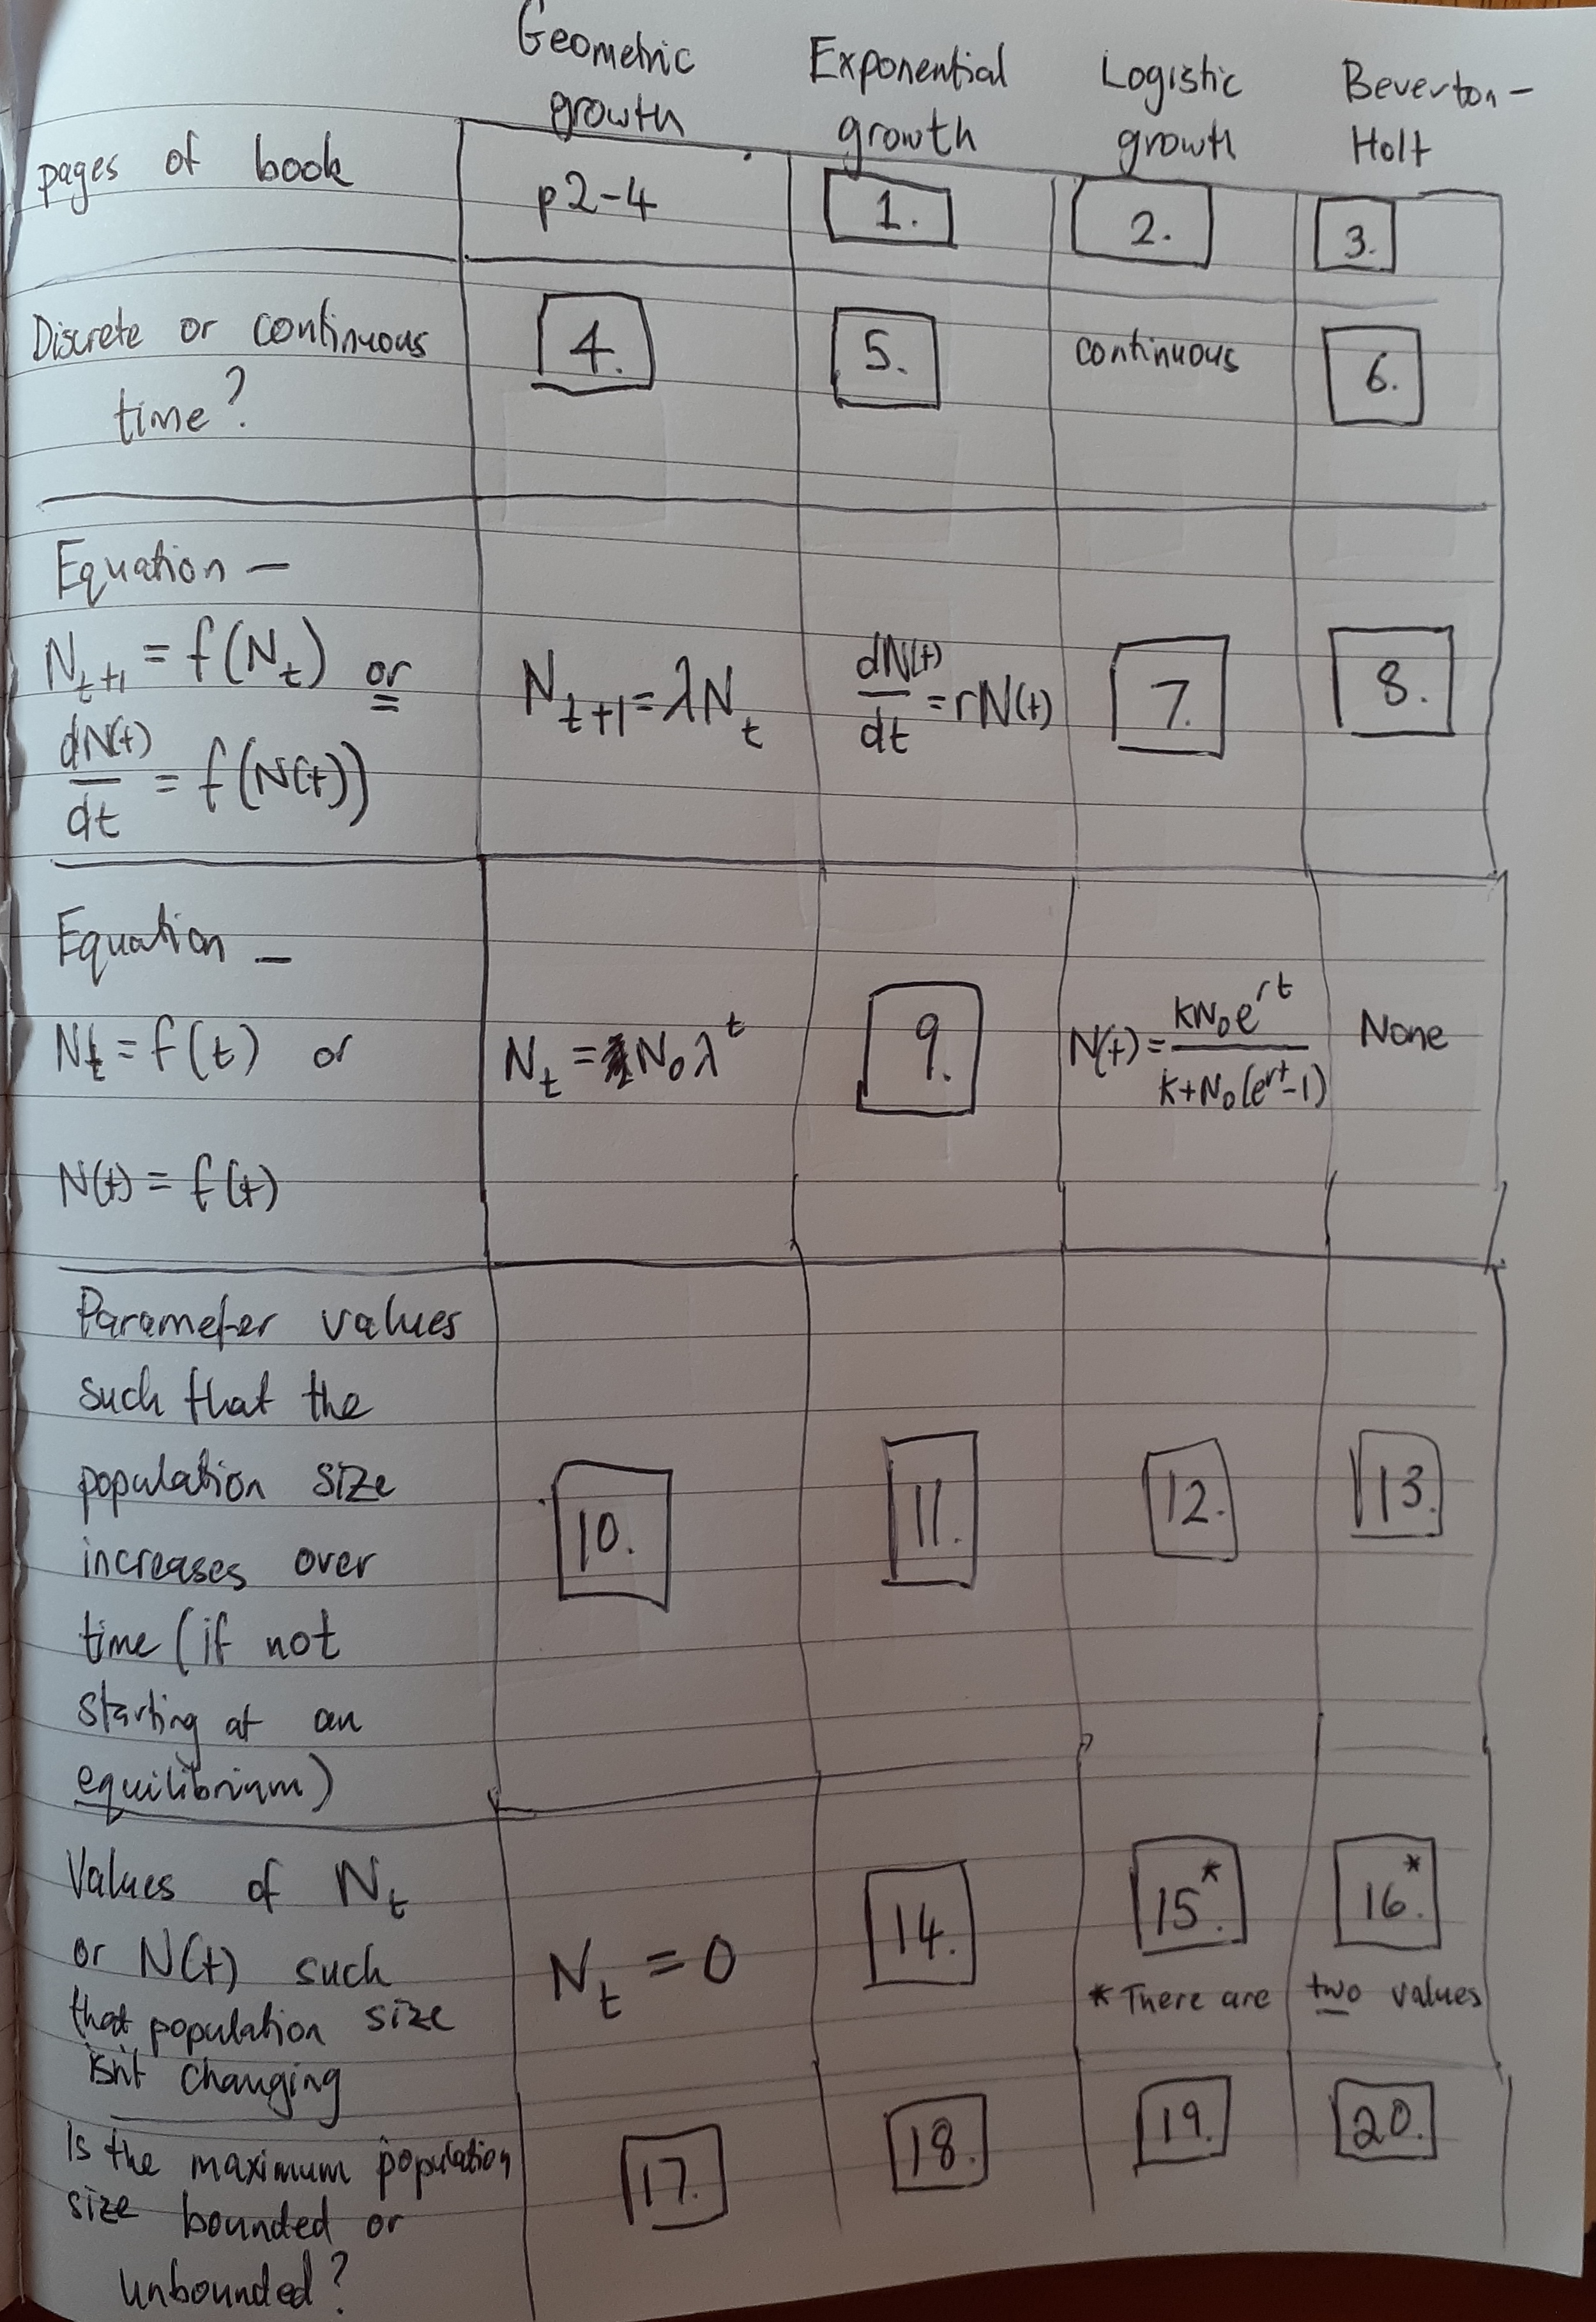
\includegraphics[width=1.2\linewidth]{figures/midterm} \caption{If this table is difficult to read, please ask Dr. Hurford for clarification}\label{fig:midterm}
\end{figure}

\section{Chapter 6 in Sherratt and
Wikinson}\label{chapter-6-in-sherratt-and-wikinson}

Chapter 6. \emph{Is Nature Chaotic} of Big problems in ecology and
evolution by Sherratt and Wilkinson.
\href{https://ebookcentral.proquest.com/lib/mun/reader.action?docID=430616\&ppg=136}{Link}

\begin{enumerate}
\def\labelenumi{\arabic{enumi}.}
\item
  What is chaos? {[}1 mark{]}
\item
  Write down a population model that produces chaos? Define all the
  parameters and variables in the model. {[}4 marks{]}
\item
  For the population model from your previous answer, for what values of
  the parameters does chaos occur? {[}1 mark{]}
\item
  What is the butterfly effect? {[}1 mark{]}
\item
  Give one example of a laboratory experiment that showed evidence of
  chaos. List one limitation of this experiment. Provide the full
  citation. {[}3 marks{]}
\item
  Give one natural (non-laboratory) example of a population that may
  show chaotic dynamics. List one limitation of this study. Provide the
  full citation. {[}3 marks{]}
\item
  Overall, based on Sherratt and Wilkinson, is there evidence that
  biological populations exhibit chaotic dynamics? {[}1 mark{]}
\end{enumerate}

\section{p30-36 in Vandermeer and
Goldberg}\label{p30-36-in-vandermeer-and-goldberg}

Vandermeer, J.H., Goldberg, D.E., 2013. Population Ecology: First
Principles (Second Edition). Princeton University Press, Princeton,
United States. p30-36.
\href{https://ebookcentral-proquest-com.qe2a-proxy.mun.ca/lib/mun/detail.action?docID=1205619}{Link}

\begin{enumerate}
\def\labelenumi{\arabic{enumi}.}
\item
  What is the stable age distribution? {[}1 mark{]}
\item
  What type of growth do the matrix population models described on
  p30-36 have? {[}1 mark{]}
\item
  How can the finite rate of increase of the population be calcuated
  when the population is described by the matrix population models
  described on p30-36? {[}1 mark{]}
\item
  For a 2 \(\times\) 2 projection matrix,
\end{enumerate}

\begin{equation}
\mathbb{P} = 
\left[
\begin{array}{cc}
p_{11} & p_{12} \\
p_{21} & p_{22} \\
\end{array}
\right],
\end{equation}

the eigenvalues are calculated by solving,

\begin{equation}
0 = (p_{11} - \lambda)(p_{22}-\lambda) - p_{12}p_{21}.
\end{equation}

If you expand the parenthesis (i.e.~using the
\href{https://en.wikipedia.org/wiki/FOIL_method}{FOIL method}), you will
see that the equation can be solved using the
\href{https://en.wikipedia.org/wiki/Quadratic_formula}{quadratic
formula}.

Consider the projection matrix:

\begin{equation}
\mathbb{A} = 
\left[
\begin{array}{cc}
0.1 & 2 \\
0.7 & 0.5 \\
\end{array}
\right].
\end{equation}

Calculate the two eigenvalues for this projection matrix,
\(\mathbb{A}\). {[}3 marks{]}

\begin{enumerate}
\def\labelenumi{\arabic{enumi}.}
\setcounter{enumi}{4}
\tightlist
\item
  The dominant eigenvalue value is the one that has largest absolute
  value (i.e., if \(\lambda_1 < 0\) then \(|\lambda_1| = -\lambda_1\)
  and if \(\lambda_1 >0\) then \(|\lambda_1| = \lambda_1\)).
\end{enumerate}

What is the dominant eigenvalue for the projection matrix
\(\mathbb{A}\)? {[}1 mark{]}

\begin{enumerate}
\def\labelenumi{\arabic{enumi}.}
\setcounter{enumi}{5}
\tightlist
\item
  If the absolute value of the dominant eigenvalue of a projection
  matrix is greater than 1, then the population will increase over time.
  Will the population described by the projection matrix,
  \(\mathbb{A}\), increase over time? {[}1 mark{]}
\end{enumerate}

\section{Kendall et al. 2019}\label{kendall-et-al.-2019}

Kendall et al. 2019. Persistent problems in the construction of matrix
population models. Ecological Modelling
\href{https://www.sciencedirect.com/science/article/pii/S0304380019301085}{Link}

\begin{enumerate}
\def\labelenumi{\arabic{enumi}.}
\item
  What are the 3 errors commonly encountered in matrix population
  models? {[}1 mark{]}
\item
  What is a post-breeding census? {[}1 mark{]}
\item
  Give a precise definition of \(b_x, b_i, \sigma_x\) and \(\sigma_i\).
  {[}2 marks{]}
\item
  In figure 2d of Kendall et al. 2019, juveniles are shown as
  reproducing. Is this an error? How is this related to census timing?
  {[}2 marks{]}
\item
  If you wanted to aggregrate across ages to make a stage-structured
  version of an age-structured model what section of this article would
  you consult? What is meant by age-distribution within a stage? {[}2
  marks{]}
\end{enumerate}

\section{Numerical solutions of an ordinary differential
equation.}\label{numerical-solutions-of-an-ordinary-differential-equation.}

Consider the following equation which is similar to logistic growth
except that density dependence is assumed in mortality only and is
assumed to have an exponential rather than a linear form:

\begin{equation}
\frac{dN(t)}{dt} = bN(t) - dN(t)e^{\delta N(t)}.
\end{equation}

Here, \(N(t)\) is the population density, \(b>0\) is a per captia birth
rate, \(d > 0\) is the per capita mortality rate when \(N(t)\) is small,
and \(\delta >0\) is a coefficient affecting the strength of density
dependence.

\begin{enumerate}
\def\labelenumi{\arabic{enumi}.}
\tightlist
\item
  Solve this ordinary differential equation in \texttt{R}. You are to
  hand in your R Script and a figure of the population density (y-axis)
  versus time (x-axis) with a figure caption. See \ref{figures} and
  \ref{RScript} for expectations for \texttt{R} scripts, figures and
  captions. You may want to refer to Chapter \ref{NumSolve2} for a
  template for how this problem could be solved. {[}7 marks{]}
\end{enumerate}

\chapter{Thurs Nov 5: Evolutionary
ecology}\label{thurs-nov-5-evolutionary-ecology}

DUE DATE: Thursday Nov 12.

This \href{https://www.zoology.ubc.ca/~bio418/}{link} contains the
course information for an evolutionary ecology class at UBC.

\section{Questions}\label{questions}

\begin{enumerate}
\def\labelenumi{\arabic{enumi}.}
\tightlist
\item
  Choose one of the topics and read enough about that topic to be able
  to write 1 paragraph explaining what that topic is about. Please make
  sure that your paragraph includes clear definitions of the relevant
  terms.
\end{enumerate}

List the sources of information that you read to learn about the topic.
You may choose the UBC lecture slides, the UBC readings, Wikipedia,
books from the library on evolutionary ecology, or peer-reviewed journal
articles.

{[}10 marks{]}

\section{Some relevant textbooks}\label{some-relevant-textbooks}

Big problems in ecology and evolution by Sherratt and Wilkinson.
\href{https://ebookcentral.proquest.com/lib/mun/reader.action?docID=430616\&ppg=136}{Link}.

Evolutionary ecology: concepts and case studies by Fox, Roff, and
Fairbairn
\href{https://ebookcentral-proquest-com.qe2a-proxy.mun.ca/lib/mun/detail.action?docID=430289}{Link}

\chapter{Fri Nov 6: Evolutionary
ecology}\label{fri-nov-6-evolutionary-ecology}

DUE DATE: Fri Nov 13

\section{Required reading}\label{required-reading}

Otto, Sarah P., and Troy Day. 2007. A Biologist's Guide to Mathematical
Modeling in Ecology and Evolution, Princeton University Press. Beginning
at 3.3 on p76 and ending at p82.
\href{https://ebookcentral-proquest-com.qe2a-proxy.mun.ca/lib/MUN/detail.action?docID=768551}{Link}.

\section{Questions}\label{questions}

\begin{enumerate}
\def\labelenumi{\arabic{enumi}.}
\item
  What are population-genetic models? {[}1 mark{]}
\item
  Consider the definition of
  \href{https://en.wikipedia.org/wiki/Population_dynamics}{population
  dynamics}. How are population dynamics related to population-genetic
  models? You will need to mention inheritance in your answer. {[}2
  marks{]}
\item
  What type of population growth is described by equations 3.6a and
  3.6b? {[}1 mark{]}
\item
  Typically, in this course, we have used \(\lambda\) to be the
  geometric growth rate. What are \(W_A\) and \(W_a\) in equations 3.6a
  and b, and for what values of \(W_A\) and \(W_a\) is the number of
  individuals with the \(A\) and \(a\) alleles increasing? {[}2 marks{]}
\item
  What are \(n_A(t)\) and \(n_a(t)\) in equations 3.6a and b? {[}1
  mark{]}
\item
  What formula would you use to calculate the frequency of the \(A\)
  allele at time, \(t\)? {[}1 mark{]}
\item
  Give \emph{two} versions of a formula that you would use to calculate
  the frequency of the allele \(A\) at time, \(t+1\)? {[}2 marks{]}
\item
  In equation 3.8d, what is \(p(t+1)\) and what is \(V_A\)? {[}1 mark{]}
\item
  If \(V_A > 1\), what does this imply about the geometric growth rates
  for individuals that inherit the \(A\) allele relative to those that
  inherit the \(a\) allele? {[}1 mark{]}
\item
  Using calculus, the author's derive a continuous time equation (3.11b)
  from the discrete time equation 3.8d. What is the formula for \(s_c\)?
  Provide the meaning of all parameters in your equation for \(s_c\).
  {[}2 marks{]}
\item
  Although not provided in the book, for the continuous time version of
  this population-genetic model, the equations for the number of
  individuals with each allele would be,
\end{enumerate}

\begin{eqnarray}
\frac{dn_A(t)}{dt} & = & r_A n_A(t) \\
\frac{dn_a(t)}{dt} & = & r_a n_a(t)
\end{eqnarray}

where \(r_A = b_A - d_A\) and \(r_a = b_a - d_a\), with \(b_i\) the per
capita birth rate, and \(d_i\) the per capita mortality rate for each of
the \(A\) and \(a\) alleles respectively. If \(r_A > 0\) and
\(r_a > 0\), what does this imply about the change in the number of
individuals with the \(A\) and \(a\) alleles over time? {[}1 mark{]}

\begin{enumerate}
\def\labelenumi{\arabic{enumi}.}
\setcounter{enumi}{11}
\tightlist
\item
  What is \(p=p(t)\) in equation 3.11b? Assuming that
  \(0 \leq p(t) \leq 1\), for what values of \(s_c\) does \(p(t)\)
  increase? How can this condition on \(s_c\), necessary for increasing
  \(p(t)\), be understood in terms of \(r_A\) and \(r_a\)? {[}2 marks{]}
\end{enumerate}

\chapter{Tues Nov 10: Evolutionary
ecology}\label{tues-nov-10-evolutionary-ecology}

\chapter{Final project ideas}\label{final-project-ideas}

For your final project you may choose either option:

\begin{enumerate}
\def\labelenumi{\arabic{enumi}.}
\tightlist
\item
  Review paper: Read and synthesize information on a new topic in
  population and evolutionary ecology that we have not considered in
  class.
\end{enumerate}

or,

\begin{enumerate}
\def\labelenumi{\arabic{enumi}.}
\setcounter{enumi}{1}
\tightlist
\item
  Analysis: Download and visualize a dataset relevant to population and
  evolutionary ecology. Discuss your graphs in the context of a
  principle in population and evolutionary ecology.
\end{enumerate}

\section{Option 1: Review paper}\label{option-1-review-paper}

Aim to write a final project that is similar in style to a paper that
you would read in \emph{Trends in Ecology and Evolution} (TREE). The
concepts that you cover, however, do not need to be as advanced as
something that would appear in TREE. Use
\href{https://www-sciencedirect-com.qe2a-proxy.mun.ca/science/article/pii/0169534796100379?via\%3Dihub}{Dias
et al. 1996} \emph{Sources and sinks in population biology} as a guide
for what a final project that is a \emph{Review} should aspire to look
like.

Topic ideas:

\begin{itemize}
\item
  Population dynamics in warming environments
\item
  Population dynamics in seasonal environments
\item
  Spatial population dynamics/metepopulations
\item
  Evolution of sensence
\item
  Evolution of body size
\item
  Evolution of virulence
\item
  Any of your own ideas, that are approved by Dr.~Hurford or a teaching
  assistant.
\end{itemize}

\section{Option 2: Analysis}\label{option-2-analysis}

If you choose to do a final project that is an \emph{Analysis} you
should use some of the exercises we have completed for class as a guide
(for example, the Doubling time or Protection Island analyses - note
that you will need to write your final project as a report, rather than
a series of questions as the assignments typically are). You are
expected to subset the data and make a graph. Be sure to decide on a
principle from population biology or evolutionary ecology to discuss
your analysis with respect to. For ideas you may wish to consult
textbooks in these subject areas.

The style of your write up will be that of a regular scientific paper
that includes an analysis, for example,
\href{https://www.pnas.org/content/110/11/4230}{Suweis et al. 2013}:
\emph{The water-controlled wealth of nations}.

Some examples of data sources are:

\begin{itemize}
\item
  The \href{https://portal.edirepository.org/nis/home.jsp}{Environmental
  Data Initiative}
\item
  \href{https://portal.edirepository.org/nis/metadataviewer?packageid=knb-lter-luq.96.2410865}{Canopy
  arthropod dynamics from 1991-2017 at El Verde, Puerto Rico}
\item
  \href{https://portal.edirepository.org/nis/mapbrowse?packageid=knb-lter-nin.2.1}{Zooplankton
  species in North Inlet Estuary, North Carolina}
\item
  \emph{Ghosts of Habitats Past: Environmental Carry-Over Effects Drive
  Population Dynamics in Novel Habitat} by Benjamin G. Van Allen and
  Volker H. W. Rudolf in The American Naturalist.
  \href{https://www.journals.uchicago.edu/doi/10.1086/670127?mobileUi=0}{{[}Article{]}}
  \href{https://datadryad.org/stash/dataset/doi:10.5061/dryad.t4g3r}{{[}Data{]}}
\item
  The Yellow columbine (\emph{Aquilegia chrysantha}) dataset associated
  with the
  \href{https://cran.r-project.org/web/packages/popbio/index.html}{\texttt{popbio}
  package} for \texttt{R}. See \texttt{aq.census}.
\item
  \href{https://www.pwrc.usgs.gov/BBS/RawData/}{Northern American
  Breeding Bird Survey}
\item
  \href{https://portal.edirepository.org/nis/mapbrowse?packageid=knb-lter-cwt.3026.13}{Fish
  populations in two small Appalachian streams}
\item
  \href{https://portal.edirepository.org/nis/mapbrowse?packageid=knb-lter-sev.106.214968}{Grasshopper
  Dynamics for the Sevilleta National Wildlife Refuge, New Mexico}
\item
  \href{https://apps.who.int/gho/data/node.ebola-sitrep.quick-downloads?lang=en}{Ebola
  data}
\item
  Or any of your own sources for population and evolutionary ecology
  data that you find.
\end{itemize}

\section{How to read scientific
papers}\label{how-to-read-scientific-papers}

Please consult
\href{https://www.research4life.org/blog/how-to-read-a-scientific-paper/}{How
to Read a Scientific Paper (2014)} for the recommended approach to
`reading' journal articles. Steps 1,2, and 4 are good advice, but step 3
may not be relevant for some readings.

\section{Grading Rubric: Both Review and Analysis {[}55
marks{]}}\label{grading-rubric-both-review-and-analysis-55-marks}

\begin{enumerate}
\def\labelenumi{\arabic{enumi}.}
\item
  The topic selected is within the scope of Population biology or
  evolutionary ecology. {[}5 marks{]}
\item
  The abstract follows
  \href{https://www.google.com/url?sa=t\&rct=j\&q=\&esrc=s\&source=web\&cd=\&ved=2ahUKEwjH9pDIya_sAhXig-AKHcB3BusQFjAAegQIBhAC\&url=http\%3A\%2F\%2Fwww.cbs.umn.edu\%2Fsites\%2Fdefault\%2Ffiles\%2Fpublic\%2Fdownloads\%2FAnnotated_Nature_abstract.pdf\&usg=AOvVaw2FzVPRcUQOUX2zEJXld9LQ}{this}
  format. {[}5 marks{]}
\item
  There is at least one paragraph towards the beginning of manuscript
  the overviews that main points that will be made. {[}5 marks{]}
\item
  At least 6 peer-reviewed articles are cited. {[}5 marks{]}
\item
  Citation format is consistent with the
  \href{https://www.journals.uchicago.edu/journals/an/instruct?mobileUi=0\#manuscript-format}{\emph{The
  American Naturalist}} {[}5 marks{]}
\item
  Presentation, i.e., spelling, grammar etc. {[}5 marks{]}
\item
  The last paragraph or section of the report summarizes the main point.
  {[}5 points{]}
\item
  There is at least one figure or table, and these include a figure
  caption. {[}20 marks{]}
\end{enumerate}

\subsection{Grading Rubric: Review only {[}55
marks{]}}\label{grading-rubric-review-only-55-marks}

\begin{enumerate}
\def\labelenumi{\arabic{enumi}.}
\item
  The report is organized into sections. Each section has a clear point.
  {[}5 marks{]}
\item
  All sections together make a cohesive unit. {[}10 marks{]}
\item
  The citations are discussed in a way that demonstrates understanding
  of their content. {[}10 marks{]}
\item
  The citations are synthesized into a cohesive narrative. {[}10
  marks{]}
\item
  Claims are fully supported by citations. {[}5 marks{]}
\item
  The report makes a clear point {[}5 marks{]}
\item
  The report provides an insightful narrative - arising from a thorough
  reading of the relevant peer-reviewed literature. {[}10 marks{]}
\end{enumerate}

\subsection{Grading Rubric: Analysis only {[}55
marks{]}}\label{grading-rubric-analysis-only-55-marks}

\begin{enumerate}
\def\labelenumi{\arabic{enumi}.}
\item
  An R Script that makes the figures in the report. {[}15 marks{]}
\item
  Report is organized into sections: 1) Introduction; 2) Data; 3)
  Analysis; and 4) Discussion. {[}5 marks{]}
\item
  The Introduction describes principles in population biology or
  evolutionary ecology and describes a hypothesis to be considered in
  light of the data visualization. {[}10 marks{]}
\item
  The Data section describes the dataset that will be analyzed and
  provides a link to where the data can be accessed. {[}5 marks{]}
\item
  Sufficient details are provided so that it is possible to evaluate the
  agreement between the formulation of the hypothesis and the data
  visualization that was done. {[}10 marks{]}
\item
  The Discussion outlines limitations of the analysis. If you would have
  liked to do another visualization or statistical analysis but do not
  know how to do it, mention this in the discussion - you will receive
  credit for having ideas of what to do, even if currently you don't
  know how to do it. {[}10 marks{]}
\end{enumerate}

\backmatter

\end{document}
